\documentclass[twoside]{book}

% Packages required by doxygen
\usepackage{fixltx2e}
\usepackage{calc}
\usepackage{doxygen}
\usepackage[export]{adjustbox} % also loads graphicx
\usepackage{graphicx}
\usepackage[utf8]{inputenc}
\usepackage{makeidx}
\usepackage{multicol}
\usepackage{multirow}
\PassOptionsToPackage{warn}{textcomp}
\usepackage{textcomp}
\usepackage[nointegrals]{wasysym}
\usepackage[table]{xcolor}

% Font selection
\usepackage[T1]{fontenc}
\usepackage[scaled=.90]{helvet}
\usepackage{courier}
\usepackage{amssymb}
\usepackage{sectsty}
\renewcommand{\familydefault}{\sfdefault}
\allsectionsfont{%
  \fontseries{bc}\selectfont%
  \color{darkgray}%
}
\renewcommand{\DoxyLabelFont}{%
  \fontseries{bc}\selectfont%
  \color{darkgray}%
}
\newcommand{\+}{\discretionary{\mbox{\scriptsize$\hookleftarrow$}}{}{}}

% Page & text layout
\usepackage{geometry}
\geometry{%
  a4paper,%
  top=2.5cm,%
  bottom=2.5cm,%
  left=2.5cm,%
  right=2.5cm%
}
\tolerance=750
\hfuzz=15pt
\hbadness=750
\setlength{\emergencystretch}{15pt}
\setlength{\parindent}{0cm}
\setlength{\parskip}{0.2cm}
\makeatletter
\renewcommand{\paragraph}{%
  \@startsection{paragraph}{4}{0ex}{-1.0ex}{1.0ex}{%
    \normalfont\normalsize\bfseries\SS@parafont%
  }%
}
\renewcommand{\subparagraph}{%
  \@startsection{subparagraph}{5}{0ex}{-1.0ex}{1.0ex}{%
    \normalfont\normalsize\bfseries\SS@subparafont%
  }%
}
\makeatother

% Headers & footers
\usepackage{fancyhdr}
\pagestyle{fancyplain}
\fancyhead[LE]{\fancyplain{}{\bfseries\thepage}}
\fancyhead[CE]{\fancyplain{}{}}
\fancyhead[RE]{\fancyplain{}{\bfseries\leftmark}}
\fancyhead[LO]{\fancyplain{}{\bfseries\rightmark}}
\fancyhead[CO]{\fancyplain{}{}}
\fancyhead[RO]{\fancyplain{}{\bfseries\thepage}}
\fancyfoot[LE]{\fancyplain{}{}}
\fancyfoot[CE]{\fancyplain{}{}}
\fancyfoot[RE]{\fancyplain{}{\bfseries\scriptsize Generated on Thu Jun 16 2016 15\+:01\+:34 for Communication Protocols by Doxygen }}
\fancyfoot[LO]{\fancyplain{}{\bfseries\scriptsize Generated on Thu Jun 16 2016 15\+:01\+:34 for Communication Protocols by Doxygen }}
\fancyfoot[CO]{\fancyplain{}{}}
\fancyfoot[RO]{\fancyplain{}{}}
\renewcommand{\footrulewidth}{0.4pt}
\renewcommand{\chaptermark}[1]{%
  \markboth{#1}{}%
}
\renewcommand{\sectionmark}[1]{%
  \markright{\thesection\ #1}%
}

% Indices & bibliography
\usepackage{natbib}
\usepackage[titles]{tocloft}
\setcounter{tocdepth}{3}
\setcounter{secnumdepth}{5}
\makeindex

% Hyperlinks (required, but should be loaded last)
\usepackage{ifpdf}
\ifpdf
  \usepackage[pdftex,pagebackref=true]{hyperref}
\else
  \usepackage[ps2pdf,pagebackref=true]{hyperref}
\fi
\hypersetup{%
  colorlinks=true,%
  linkcolor=blue,%
  citecolor=blue,%
  unicode%
}

% Custom commands
\newcommand{\clearemptydoublepage}{%
  \newpage{\pagestyle{empty}\cleardoublepage}%
}


%===== C O N T E N T S =====

\begin{document}

% Titlepage & ToC
\hypersetup{pageanchor=false,
             bookmarks=true,
             bookmarksnumbered=true,
             pdfencoding=unicode
            }
\pagenumbering{roman}
\begin{titlepage}
\vspace*{7cm}
\begin{center}%
{\Large Communication Protocols \\[1ex]\large 1.\+0 }\\
\vspace*{1cm}
{\large Generated by Doxygen 1.8.9.1}\\
\vspace*{0.5cm}
{\small Thu Jun 16 2016 15:01:34}\\
\end{center}
\end{titlepage}
\clearemptydoublepage
\tableofcontents
\clearemptydoublepage
\pagenumbering{arabic}
\hypersetup{pageanchor=true}

%--- Begin generated contents ---
\chapter{Module Index}
\section{Modules}
Here is a list of all modules\+:\begin{DoxyCompactList}
\item \contentsline{section}{Comminucation\+Protocols}{\pageref{group___comminucation_protocols}}{}
\end{DoxyCompactList}

\chapter{Hierarchical Index}
\section{Class Hierarchy}
This inheritance list is sorted roughly, but not completely, alphabetically\+:\begin{DoxyCompactList}
\item \contentsline{section}{Application\+Protocol}{\pageref{class_application_protocol}}{}
\begin{DoxyCompactList}
\item \contentsline{section}{Qik}{\pageref{class_qik}}{}
\item \contentsline{section}{Rest\+Application\+Protocol}{\pageref{class_rest_application_protocol}}{}
\end{DoxyCompactList}
\item exception\begin{DoxyCompactList}
\item \contentsline{section}{Connection\+Exception}{\pageref{class_connection_exception}}{}
\end{DoxyCompactList}
\item thread\begin{DoxyCompactList}
\item \contentsline{section}{T\+C\+P\+Socket}{\pageref{class_t_c_p_socket}}{}
\item \contentsline{section}{U\+A\+R\+T}{\pageref{class_u_a_r_t}}{}
\end{DoxyCompactList}
\item \contentsline{section}{Transport\+Listener}{\pageref{class_transport_listener}}{}
\begin{DoxyCompactList}
\item \contentsline{section}{Qik}{\pageref{class_qik}}{}
\item \contentsline{section}{Rest\+Application\+Protocol}{\pageref{class_rest_application_protocol}}{}
\end{DoxyCompactList}
\item \contentsline{section}{Transport\+Protocol}{\pageref{class_transport_protocol}}{}
\begin{DoxyCompactList}
\item \contentsline{section}{T\+C\+P\+Socket}{\pageref{class_t_c_p_socket}}{}
\item \contentsline{section}{U\+A\+R\+T}{\pageref{class_u_a_r_t}}{}
\end{DoxyCompactList}
\end{DoxyCompactList}

\chapter{Class Index}
\section{Class List}
Here are the classes, structs, unions and interfaces with brief descriptions\+:\begin{DoxyCompactList}
\item\contentsline{section}{\hyperlink{class_application_protocol}{Application\+Protocol} }{\pageref{class_application_protocol}}{}
\item\contentsline{section}{\hyperlink{class_connection_exception}{Connection\+Exception} }{\pageref{class_connection_exception}}{}
\item\contentsline{section}{\hyperlink{class_qik}{Qik} }{\pageref{class_qik}}{}
\item\contentsline{section}{\hyperlink{class_rest_application_protocol}{Rest\+Application\+Protocol} }{\pageref{class_rest_application_protocol}}{}
\item\contentsline{section}{\hyperlink{class_t_c_p_socket}{T\+C\+P\+Socket} }{\pageref{class_t_c_p_socket}}{}
\item\contentsline{section}{\hyperlink{class_transport_listener}{Transport\+Listener} }{\pageref{class_transport_listener}}{}
\item\contentsline{section}{\hyperlink{class_transport_protocol}{Transport\+Protocol} }{\pageref{class_transport_protocol}}{}
\item\contentsline{section}{\hyperlink{class_u_a_r_t}{U\+A\+R\+T} }{\pageref{class_u_a_r_t}}{}
\end{DoxyCompactList}

\chapter{File Index}
\section{File List}
Here is a list of all documented files with brief descriptions\+:\begin{DoxyCompactList}
\item\contentsline{section}{C\+:/\+Users/koen/\+Documents/\+Git\+Hub/communication-\/protocols/source/include/\hyperlink{_application_protocol_8hpp}{Application\+Protocol.\+hpp} \\*\hyperlink{class_application_protocol}{Application\+Protocol} is used to define a type that other applications can use. Such as \hyperlink{class_qik}{Qik} and R\+E\+S\+T }{\pageref{_application_protocol_8hpp}}{}
\item\contentsline{section}{C\+:/\+Users/koen/\+Documents/\+Git\+Hub/communication-\/protocols/source/include/\hyperlink{_comport_defines_8hpp}{Comport\+Defines.\+hpp} \\*Comport\+Defines is used to define all the different comports in a cygwin (windows) system }{\pageref{_comport_defines_8hpp}}{}
\item\contentsline{section}{C\+:/\+Users/koen/\+Documents/\+Git\+Hub/communication-\/protocols/source/include/\hyperlink{_connection_exception_8hpp}{Connection\+Exception.\+hpp} \\*Exception class to make sure transportprotocols can throw exceptions }{\pageref{_connection_exception_8hpp}}{}
\item\contentsline{section}{C\+:/\+Users/koen/\+Documents/\+Git\+Hub/communication-\/protocols/source/include/\hyperlink{_qik_8hpp}{Qik.\+hpp} \\*\hyperlink{class_qik}{Qik} is a application protocol to comminucate with the Rosbee procotol \hyperlink{class_qik}{Qik} }{\pageref{_qik_8hpp}}{}
\item\contentsline{section}{C\+:/\+Users/koen/\+Documents/\+Git\+Hub/communication-\/protocols/source/include/\hyperlink{_rest_application_protocol_8hpp}{Rest\+Application\+Protocol.\+hpp} \\*\hyperlink{class_application_protocol}{Application\+Protocol} to comminucate with R\+E\+S\+T over a transport protocol }{\pageref{_rest_application_protocol_8hpp}}{}
\item\contentsline{section}{C\+:/\+Users/koen/\+Documents/\+Git\+Hub/communication-\/protocols/source/include/\hyperlink{_t_c_p_socket_8hpp}{T\+C\+P\+Socket.\+hpp} \\*\hyperlink{class_t_c_p_socket}{T\+C\+P\+Socket} is used as transportprotocol to comminucate over T\+C\+P }{\pageref{_t_c_p_socket_8hpp}}{}
\item\contentsline{section}{C\+:/\+Users/koen/\+Documents/\+Git\+Hub/communication-\/protocols/source/include/\hyperlink{_transport_listener_8hpp}{Transport\+Listener.\+hpp} \\*\hyperlink{class_transport_listener}{Transport\+Listener} is a interface to make sure some Application\+Protocols can listen to incoming data }{\pageref{_transport_listener_8hpp}}{}
\item\contentsline{section}{C\+:/\+Users/koen/\+Documents/\+Git\+Hub/communication-\/protocols/source/include/\hyperlink{_transport_protocol_8hpp}{Transport\+Protocol.\+hpp} \\*A default interface for \hyperlink{class_transport_protocol}{Transport\+Protocol} to make sure }{\pageref{_transport_protocol_8hpp}}{}
\item\contentsline{section}{C\+:/\+Users/koen/\+Documents/\+Git\+Hub/communication-\/protocols/source/include/\hyperlink{_u_a_r_t_8hpp}{U\+A\+R\+T.\+hpp} \\*\hyperlink{class_u_a_r_t}{U\+A\+R\+T} is a protocol to transfer data via a serial interface }{\pageref{_u_a_r_t_8hpp}}{}
\end{DoxyCompactList}

\chapter{Module Documentation}
\hypertarget{group___comminucation_protocols}{}\section{Comminucation\+Protocols}
\label{group___comminucation_protocols}\index{Comminucation\+Protocols@{Comminucation\+Protocols}}


Defines different commincation protocols for embedded systems.  


Defines different commincation protocols for embedded systems. 

Comminucation\+Protocol is a project to determine the different ways embedded systems can comminucate with each other. 
\chapter{Class Documentation}
\hypertarget{class_application_protocol}{}\section{Application\+Protocol Class Reference}
\label{class_application_protocol}\index{Application\+Protocol@{Application\+Protocol}}


{\ttfamily \#include $<$Application\+Protocol.\+hpp$>$}

Inheritance diagram for Application\+Protocol\+:\begin{figure}[H]
\begin{center}
\leavevmode
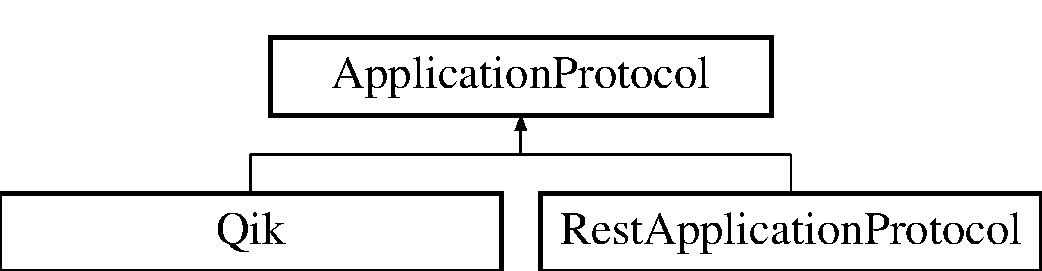
\includegraphics[height=2.000000cm]{class_application_protocol}
\end{center}
\end{figure}
\subsection*{Public Member Functions}
\begin{DoxyCompactItemize}
\item 
\hyperlink{class_application_protocol_ae2a832cc8ffb74ede5582471187f2da1}{Application\+Protocol} (\hyperlink{class_transport_protocol}{Transport\+Protocol} \&t)
\item 
void \hyperlink{class_application_protocol_a6005c829686a0040803063aaea9d84ae}{set\+Transport\+Protocol} (\hyperlink{class_transport_protocol}{Transport\+Protocol} \&t)
\end{DoxyCompactItemize}
\subsection*{Protected Attributes}
\begin{DoxyCompactItemize}
\item 
\hypertarget{class_application_protocol_a7e626f0d9d9df956ef38737939a6d1c0}{}\hyperlink{class_transport_protocol}{Transport\+Protocol} \& {\bfseries transport}\label{class_application_protocol_a7e626f0d9d9df956ef38737939a6d1c0}

\end{DoxyCompactItemize}


\subsection{Detailed Description}
An abstract class used to create a wrapper around a Applicaion Protocol. \begin{DoxyAuthor}{Author}
Koen van der Kruk, 
\end{DoxyAuthor}
\begin{DoxyVersion}{Version}
1.\+0 
\end{DoxyVersion}
\begin{DoxyDate}{Date}
8-\/6-\/2016 
\end{DoxyDate}


\subsection{Constructor \& Destructor Documentation}
\hypertarget{class_application_protocol_ae2a832cc8ffb74ede5582471187f2da1}{}\index{Application\+Protocol@{Application\+Protocol}!Application\+Protocol@{Application\+Protocol}}
\index{Application\+Protocol@{Application\+Protocol}!Application\+Protocol@{Application\+Protocol}}
\subsubsection[{Application\+Protocol}]{\setlength{\rightskip}{0pt plus 5cm}Application\+Protocol\+::\+Application\+Protocol (
\begin{DoxyParamCaption}
\item[{{\bf Transport\+Protocol} \&}]{t}
\end{DoxyParamCaption}
)\hspace{0.3cm}{\ttfamily [inline]}}\label{class_application_protocol_ae2a832cc8ffb74ede5582471187f2da1}
Constructor to initialize a apllication protocol containing a transport protocol. 
\begin{DoxyParams}{Parameters}
{\em t} & The transportprotocol used to transfer the data between multiple nodes \\
\hline
\end{DoxyParams}


\subsection{Member Function Documentation}
\hypertarget{class_application_protocol_a6005c829686a0040803063aaea9d84ae}{}\index{Application\+Protocol@{Application\+Protocol}!set\+Transport\+Protocol@{set\+Transport\+Protocol}}
\index{set\+Transport\+Protocol@{set\+Transport\+Protocol}!Application\+Protocol@{Application\+Protocol}}
\subsubsection[{set\+Transport\+Protocol}]{\setlength{\rightskip}{0pt plus 5cm}void Application\+Protocol\+::set\+Transport\+Protocol (
\begin{DoxyParamCaption}
\item[{{\bf Transport\+Protocol} \&}]{t}
\end{DoxyParamCaption}
)\hspace{0.3cm}{\ttfamily [inline]}}\label{class_application_protocol_a6005c829686a0040803063aaea9d84ae}
Can be used to change the \hyperlink{class_transport_protocol}{Transport\+Protocol} after the object is already initiliazed 
\begin{DoxyParams}{Parameters}
{\em t} & The \hyperlink{class_transport_protocol}{Transport\+Protocol} used to transfer data between nodes. \\
\hline
\end{DoxyParams}


The documentation for this class was generated from the following file\+:\begin{DoxyCompactItemize}
\item 
C\+:/\+Users/koen/\+Documents/\+Git\+Hub/communication-\/protocols/source/include/\hyperlink{_application_protocol_8hpp}{Application\+Protocol.\+hpp}\end{DoxyCompactItemize}

\hypertarget{class_connection_exception}{}\section{Connection\+Exception Class Reference}
\label{class_connection_exception}\index{Connection\+Exception@{Connection\+Exception}}


{\ttfamily \#include $<$Connection\+Exception.\+hpp$>$}

Inheritance diagram for Connection\+Exception\+:\begin{figure}[H]
\begin{center}
\leavevmode
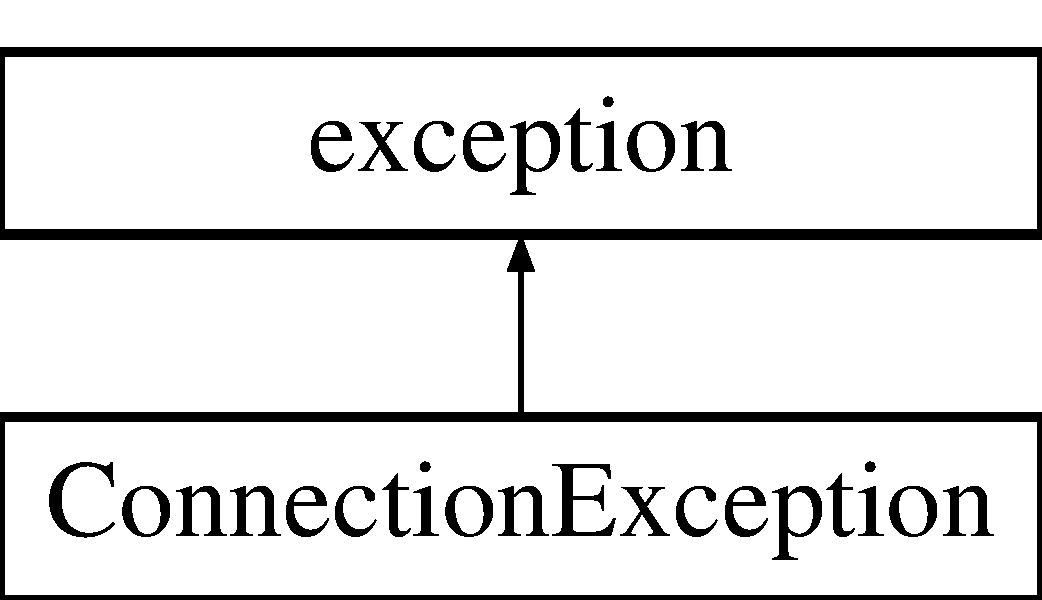
\includegraphics[height=2.000000cm]{class_connection_exception}
\end{center}
\end{figure}
\subsection*{Public Member Functions}
\begin{DoxyCompactItemize}
\item 
\hyperlink{class_connection_exception_ab4dd2e1058fb571fce2f9fea06a61403}{Connection\+Exception} (std\+::string arg)
\item 
virtual const char $\ast$ \hyperlink{class_connection_exception_a046e901d8e5fd6a893ae13640fab21bf}{what} () const   throw ()
\end{DoxyCompactItemize}


\subsection{Detailed Description}
An abstract class used to create a wrapper around a Applicaion Protocol. \begin{DoxyAuthor}{Author}
Thijs Hendrickx 
\end{DoxyAuthor}
\begin{DoxyVersion}{Version}
1.\+0 
\end{DoxyVersion}
\begin{DoxyDate}{Date}
16-\/6-\/2016 
\end{DoxyDate}


\subsection{Constructor \& Destructor Documentation}
\hypertarget{class_connection_exception_ab4dd2e1058fb571fce2f9fea06a61403}{}\index{Connection\+Exception@{Connection\+Exception}!Connection\+Exception@{Connection\+Exception}}
\index{Connection\+Exception@{Connection\+Exception}!Connection\+Exception@{Connection\+Exception}}
\subsubsection[{Connection\+Exception}]{\setlength{\rightskip}{0pt plus 5cm}Connection\+Exception\+::\+Connection\+Exception (
\begin{DoxyParamCaption}
\item[{std\+::string}]{arg}
\end{DoxyParamCaption}
)\hspace{0.3cm}{\ttfamily [inline]}}\label{class_connection_exception_ab4dd2e1058fb571fce2f9fea06a61403}
Constructor to create a connection exception. 
\begin{DoxyParams}{Parameters}
{\em arg} & The message for the exception \\
\hline
\end{DoxyParams}


\subsection{Member Function Documentation}
\hypertarget{class_connection_exception_a046e901d8e5fd6a893ae13640fab21bf}{}\index{Connection\+Exception@{Connection\+Exception}!what@{what}}
\index{what@{what}!Connection\+Exception@{Connection\+Exception}}
\subsubsection[{what}]{\setlength{\rightskip}{0pt plus 5cm}virtual const char$\ast$ Connection\+Exception\+::what (
\begin{DoxyParamCaption}
{}
\end{DoxyParamCaption}
) const throw  ) \hspace{0.3cm}{\ttfamily [inline]}, {\ttfamily [virtual]}}\label{class_connection_exception_a046e901d8e5fd6a893ae13640fab21bf}
Virtual method to throw connection exception \begin{DoxyReturn}{Returns}
The const char containing the exception message. 
\end{DoxyReturn}


The documentation for this class was generated from the following file\+:\begin{DoxyCompactItemize}
\item 
C\+:/\+Users/koen/\+Documents/\+Git\+Hub/communication-\/protocols/source/include/\hyperlink{_connection_exception_8hpp}{Connection\+Exception.\+hpp}\end{DoxyCompactItemize}

\hypertarget{class_qik}{}\section{Qik Class Reference}
\label{class_qik}\index{Qik@{Qik}}
Inheritance diagram for Qik\+:\begin{figure}[H]
\begin{center}
\leavevmode
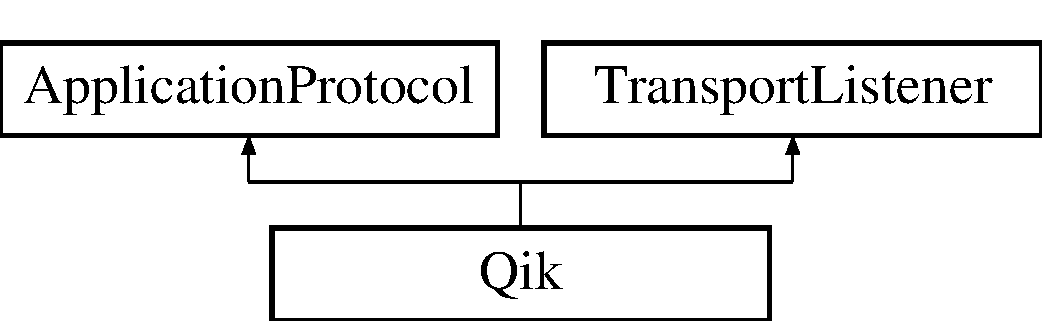
\includegraphics[height=2.000000cm]{class_qik}
\end{center}
\end{figure}
\subsection*{Public Member Functions}
\begin{DoxyCompactItemize}
\item 
\hyperlink{class_qik_a40dc67c7d28bb8e5148fa459795482b3}{Qik} (\hyperlink{class_transport_protocol}{Transport\+Protocol} \&t)
\begin{DoxyCompactList}\small\item\em Constructor of the \hyperlink{class_qik}{Qik} Application protocol. \end{DoxyCompactList}\item 
void \hyperlink{class_qik_a0104c2a0c22fbbf83de456cc7cb9840d}{data\+\_\+received} (uint8\+\_\+t $\ast$data, int number\+\_\+of\+\_\+bytes) override
\item 
uint8\+\_\+t \hyperlink{class_qik_adb551278953edfda128886a9df14e986}{get\+\_\+firmware\+\_\+version} ()
\begin{DoxyCompactList}\small\item\em reads the frimwareversion from the \hyperlink{class_qik}{Qik}. \end{DoxyCompactList}\item 
uint8\+\_\+t \hyperlink{class_qik_ad65a5d6fbdfde7998b4ef537ad07b843}{get\+\_\+errors} ()
\begin{DoxyCompactList}\small\item\em reads the Errors from the \hyperlink{class_qik}{Qik}. \end{DoxyCompactList}\item 
uint8\+\_\+t \hyperlink{class_qik_a8b4e0f9f0c42cc812f9ead37a766e5ff}{get\+\_\+configuration\+\_\+parameter} (uint8\+\_\+t parameter)
\begin{DoxyCompactList}\small\item\em reads the configurated parameter from the qik; \end{DoxyCompactList}\item 
\hypertarget{class_qik_a6201e2e6a24997827aefd2eac20524f6}{}uint8\+\_\+t {\bfseries set\+\_\+configuration\+\_\+parameter} (uint8\+\_\+t parameter, uint8\+\_\+t value)\label{class_qik_a6201e2e6a24997827aefd2eac20524f6}

\item 
void \hyperlink{class_qik_a6dc1b476ef343bdc6def0f6fd548002a}{set\+\_\+m0\+\_\+speed} (int speed)
\begin{DoxyCompactList}\small\item\em set the speed of motor 0 \end{DoxyCompactList}\item 
void \hyperlink{class_qik_a0973688f7c423dff7cfaa26dab91a126}{set\+\_\+m1\+\_\+speed} (int speed)
\begin{DoxyCompactList}\small\item\em set the speed of motor 1 \end{DoxyCompactList}\item 
void \hyperlink{class_qik_a6d504c59e7eec46da40ad9e71199b6ff}{set\+\_\+speeds} (int m0\+Speed, int m1\+Speed)
\begin{DoxyCompactList}\small\item\em set the speeds of motor 1 and 2 \end{DoxyCompactList}\item 
void \hyperlink{class_qik_a2b2195033a0459df0daec4a01898811a}{set\+\_\+m0\+\_\+brake} (uint8\+\_\+t brake)
\begin{DoxyCompactList}\small\item\em set the brake for motor 0 \end{DoxyCompactList}\item 
void \hyperlink{class_qik_a1795a6acae6aa0f9be0784ff408e5225}{set\+\_\+m1\+\_\+brake} (uint8\+\_\+t brake)
\begin{DoxyCompactList}\small\item\em set the brake for motor 0 \end{DoxyCompactList}\item 
void \hyperlink{class_qik_a0c6762eb5ffe8eaaa12407126caf568c}{set\+\_\+brakes} (uint8\+\_\+t m0\+Brake, uint8\+\_\+t m1\+Brake)
\begin{DoxyCompactList}\small\item\em set the brakes for motor 0 and 1 \end{DoxyCompactList}\item 
uint8\+\_\+t \hyperlink{class_qik_a73e1dfec2256dbe5d8ba2147501bf7d9}{get\+\_\+m0\+\_\+current} ()
\begin{DoxyCompactList}\small\item\em get the current of motor 0 \end{DoxyCompactList}\item 
uint8\+\_\+t \hyperlink{class_qik_a4d786f955b48b2d1a4e866ca6f3b94b8}{get\+\_\+m1\+\_\+current} ()
\begin{DoxyCompactList}\small\item\em get the current of motor 1 \end{DoxyCompactList}\item 
unsigned int \hyperlink{class_qik_a44a14db2e00629f31c2996269c856a19}{get\+\_\+m0\+\_\+current\+\_\+milliamps} ()
\begin{DoxyCompactList}\small\item\em get the current of motor 0 in milliamps \end{DoxyCompactList}\item 
unsigned int \hyperlink{class_qik_a44bb8dd4f9086e94e253ab7907080fb9}{get\+\_\+m1\+\_\+current\+\_\+milliamps} ()
\begin{DoxyCompactList}\small\item\em get the current of motor 1 in milliamps \end{DoxyCompactList}\item 
uint8\+\_\+t \hyperlink{class_qik_a8bab82a92a918d6c5f8f1aa921354fd6}{get\+\_\+m0\+\_\+speed} ()
\begin{DoxyCompactList}\small\item\em get the speed of motor 0 \end{DoxyCompactList}\item 
uint8\+\_\+t \hyperlink{class_qik_a8d37d1be0a983cf255990ee137985b1d}{get\+\_\+m1\+\_\+speed} ()
\begin{DoxyCompactList}\small\item\em get the speed of motor 1 \end{DoxyCompactList}\end{DoxyCompactItemize}
\subsection*{Additional Inherited Members}


\subsection{Constructor \& Destructor Documentation}
\hypertarget{class_qik_a40dc67c7d28bb8e5148fa459795482b3}{}\index{Qik@{Qik}!Qik@{Qik}}
\index{Qik@{Qik}!Qik@{Qik}}
\subsubsection[{Qik}]{\setlength{\rightskip}{0pt plus 5cm}Qik\+::\+Qik (
\begin{DoxyParamCaption}
\item[{{\bf Transport\+Protocol} \&}]{t}
\end{DoxyParamCaption}
)}\label{class_qik_a40dc67c7d28bb8e5148fa459795482b3}


Constructor of the \hyperlink{class_qik}{Qik} Application protocol. 


\begin{DoxyParams}{Parameters}
{\em t} & The transportprotocol that is used to send data. \\
\hline
\end{DoxyParams}


\subsection{Member Function Documentation}
\hypertarget{class_qik_a0104c2a0c22fbbf83de456cc7cb9840d}{}\index{Qik@{Qik}!data\+\_\+received@{data\+\_\+received}}
\index{data\+\_\+received@{data\+\_\+received}!Qik@{Qik}}
\subsubsection[{data\+\_\+received}]{\setlength{\rightskip}{0pt plus 5cm}void Qik\+::data\+\_\+received (
\begin{DoxyParamCaption}
\item[{uint8\+\_\+t $\ast$}]{data, }
\item[{int}]{number\+\_\+of\+\_\+bytes}
\end{DoxyParamCaption}
)\hspace{0.3cm}{\ttfamily [override]}, {\ttfamily [virtual]}}\label{class_qik_a0104c2a0c22fbbf83de456cc7cb9840d}
This function is called from the \hyperlink{class_transport_protocol}{Transport\+Protocol} to send data between multiple nodes. 
\begin{DoxyParams}{Parameters}
{\em data} & The transfered data to the listener. \\
\hline
\end{DoxyParams}


Implements \hyperlink{class_transport_listener_aafc4dd15ef03baa68b36b45c43c5addd}{Transport\+Listener}.

\hypertarget{class_qik_a8b4e0f9f0c42cc812f9ead37a766e5ff}{}\index{Qik@{Qik}!get\+\_\+configuration\+\_\+parameter@{get\+\_\+configuration\+\_\+parameter}}
\index{get\+\_\+configuration\+\_\+parameter@{get\+\_\+configuration\+\_\+parameter}!Qik@{Qik}}
\subsubsection[{get\+\_\+configuration\+\_\+parameter}]{\setlength{\rightskip}{0pt plus 5cm}uint8\+\_\+t Qik\+::get\+\_\+configuration\+\_\+parameter (
\begin{DoxyParamCaption}
\item[{uint8\+\_\+t}]{parameter}
\end{DoxyParamCaption}
)}\label{class_qik_a8b4e0f9f0c42cc812f9ead37a766e5ff}


reads the configurated parameter from the qik; 


\begin{DoxyParams}{Parameters}
{\em parameter} & the parameter in range 0-\/11 that needs to be readed; \\
\hline
\end{DoxyParams}
\begin{DoxyReturn}{Returns}
uint8\+\_\+t The value of the parameter that is readed; 
\end{DoxyReturn}
\hypertarget{class_qik_ad65a5d6fbdfde7998b4ef537ad07b843}{}\index{Qik@{Qik}!get\+\_\+errors@{get\+\_\+errors}}
\index{get\+\_\+errors@{get\+\_\+errors}!Qik@{Qik}}
\subsubsection[{get\+\_\+errors}]{\setlength{\rightskip}{0pt plus 5cm}uint8\+\_\+t Qik\+::get\+\_\+errors (
\begin{DoxyParamCaption}
{}
\end{DoxyParamCaption}
)}\label{class_qik_ad65a5d6fbdfde7998b4ef537ad07b843}


reads the Errors from the \hyperlink{class_qik}{Qik}. 

\begin{DoxyReturn}{Returns}
uint8\+\_\+t The Errorcode version that is readed. 
\end{DoxyReturn}
\hypertarget{class_qik_adb551278953edfda128886a9df14e986}{}\index{Qik@{Qik}!get\+\_\+firmware\+\_\+version@{get\+\_\+firmware\+\_\+version}}
\index{get\+\_\+firmware\+\_\+version@{get\+\_\+firmware\+\_\+version}!Qik@{Qik}}
\subsubsection[{get\+\_\+firmware\+\_\+version}]{\setlength{\rightskip}{0pt plus 5cm}uint8\+\_\+t Qik\+::get\+\_\+firmware\+\_\+version (
\begin{DoxyParamCaption}
{}
\end{DoxyParamCaption}
)}\label{class_qik_adb551278953edfda128886a9df14e986}


reads the frimwareversion from the \hyperlink{class_qik}{Qik}. 

\begin{DoxyReturn}{Returns}
uint8\+\_\+t The frimware version that is readed. 
\end{DoxyReturn}
\hypertarget{class_qik_a73e1dfec2256dbe5d8ba2147501bf7d9}{}\index{Qik@{Qik}!get\+\_\+m0\+\_\+current@{get\+\_\+m0\+\_\+current}}
\index{get\+\_\+m0\+\_\+current@{get\+\_\+m0\+\_\+current}!Qik@{Qik}}
\subsubsection[{get\+\_\+m0\+\_\+current}]{\setlength{\rightskip}{0pt plus 5cm}uint8\+\_\+t Qik\+::get\+\_\+m0\+\_\+current (
\begin{DoxyParamCaption}
{}
\end{DoxyParamCaption}
)}\label{class_qik_a73e1dfec2256dbe5d8ba2147501bf7d9}


get the current of motor 0 

\begin{DoxyReturn}{Returns}
uint8\+\_\+t the current value of motor 0 
\end{DoxyReturn}
\hypertarget{class_qik_a44a14db2e00629f31c2996269c856a19}{}\index{Qik@{Qik}!get\+\_\+m0\+\_\+current\+\_\+milliamps@{get\+\_\+m0\+\_\+current\+\_\+milliamps}}
\index{get\+\_\+m0\+\_\+current\+\_\+milliamps@{get\+\_\+m0\+\_\+current\+\_\+milliamps}!Qik@{Qik}}
\subsubsection[{get\+\_\+m0\+\_\+current\+\_\+milliamps}]{\setlength{\rightskip}{0pt plus 5cm}unsigned int Qik\+::get\+\_\+m0\+\_\+current\+\_\+milliamps (
\begin{DoxyParamCaption}
{}
\end{DoxyParamCaption}
)}\label{class_qik_a44a14db2e00629f31c2996269c856a19}


get the current of motor 0 in milliamps 

\begin{DoxyReturn}{Returns}
unsigned int the current value of motor 0 in milliamps 
\end{DoxyReturn}
\hypertarget{class_qik_a8bab82a92a918d6c5f8f1aa921354fd6}{}\index{Qik@{Qik}!get\+\_\+m0\+\_\+speed@{get\+\_\+m0\+\_\+speed}}
\index{get\+\_\+m0\+\_\+speed@{get\+\_\+m0\+\_\+speed}!Qik@{Qik}}
\subsubsection[{get\+\_\+m0\+\_\+speed}]{\setlength{\rightskip}{0pt plus 5cm}uint8\+\_\+t Qik\+::get\+\_\+m0\+\_\+speed (
\begin{DoxyParamCaption}
{}
\end{DoxyParamCaption}
)}\label{class_qik_a8bab82a92a918d6c5f8f1aa921354fd6}


get the speed of motor 0 

\begin{DoxyReturn}{Returns}
uint8\+\_\+t the speed value of motor 0 in range 0-\/255. 
\end{DoxyReturn}
\hypertarget{class_qik_a4d786f955b48b2d1a4e866ca6f3b94b8}{}\index{Qik@{Qik}!get\+\_\+m1\+\_\+current@{get\+\_\+m1\+\_\+current}}
\index{get\+\_\+m1\+\_\+current@{get\+\_\+m1\+\_\+current}!Qik@{Qik}}
\subsubsection[{get\+\_\+m1\+\_\+current}]{\setlength{\rightskip}{0pt plus 5cm}uint8\+\_\+t Qik\+::get\+\_\+m1\+\_\+current (
\begin{DoxyParamCaption}
{}
\end{DoxyParamCaption}
)}\label{class_qik_a4d786f955b48b2d1a4e866ca6f3b94b8}


get the current of motor 1 

\begin{DoxyReturn}{Returns}
uint8\+\_\+t the current value of motor 1 
\end{DoxyReturn}
\hypertarget{class_qik_a44bb8dd4f9086e94e253ab7907080fb9}{}\index{Qik@{Qik}!get\+\_\+m1\+\_\+current\+\_\+milliamps@{get\+\_\+m1\+\_\+current\+\_\+milliamps}}
\index{get\+\_\+m1\+\_\+current\+\_\+milliamps@{get\+\_\+m1\+\_\+current\+\_\+milliamps}!Qik@{Qik}}
\subsubsection[{get\+\_\+m1\+\_\+current\+\_\+milliamps}]{\setlength{\rightskip}{0pt plus 5cm}unsigned int Qik\+::get\+\_\+m1\+\_\+current\+\_\+milliamps (
\begin{DoxyParamCaption}
{}
\end{DoxyParamCaption}
)}\label{class_qik_a44bb8dd4f9086e94e253ab7907080fb9}


get the current of motor 1 in milliamps 

\begin{DoxyReturn}{Returns}
unsigned int the current value of motor 1 in milliamps 
\end{DoxyReturn}
\hypertarget{class_qik_a8d37d1be0a983cf255990ee137985b1d}{}\index{Qik@{Qik}!get\+\_\+m1\+\_\+speed@{get\+\_\+m1\+\_\+speed}}
\index{get\+\_\+m1\+\_\+speed@{get\+\_\+m1\+\_\+speed}!Qik@{Qik}}
\subsubsection[{get\+\_\+m1\+\_\+speed}]{\setlength{\rightskip}{0pt plus 5cm}uint8\+\_\+t Qik\+::get\+\_\+m1\+\_\+speed (
\begin{DoxyParamCaption}
{}
\end{DoxyParamCaption}
)}\label{class_qik_a8d37d1be0a983cf255990ee137985b1d}


get the speed of motor 1 

\begin{DoxyReturn}{Returns}
uint8\+\_\+t the speed value of motor 1 in range 0-\/255. 
\end{DoxyReturn}
\hypertarget{class_qik_a0c6762eb5ffe8eaaa12407126caf568c}{}\index{Qik@{Qik}!set\+\_\+brakes@{set\+\_\+brakes}}
\index{set\+\_\+brakes@{set\+\_\+brakes}!Qik@{Qik}}
\subsubsection[{set\+\_\+brakes}]{\setlength{\rightskip}{0pt plus 5cm}void Qik\+::set\+\_\+brakes (
\begin{DoxyParamCaption}
\item[{uint8\+\_\+t}]{m0\+Brake, }
\item[{uint8\+\_\+t}]{m1\+Brake}
\end{DoxyParamCaption}
)}\label{class_qik_a0c6762eb5ffe8eaaa12407126caf568c}


set the brakes for motor 0 and 1 


\begin{DoxyParams}{Parameters}
{\em m0\+Brake} & the brake value for motor 0 \\
\hline
{\em m1\+Brake} & the brake value for motor 1 \\
\hline
\end{DoxyParams}
\hypertarget{class_qik_a2b2195033a0459df0daec4a01898811a}{}\index{Qik@{Qik}!set\+\_\+m0\+\_\+brake@{set\+\_\+m0\+\_\+brake}}
\index{set\+\_\+m0\+\_\+brake@{set\+\_\+m0\+\_\+brake}!Qik@{Qik}}
\subsubsection[{set\+\_\+m0\+\_\+brake}]{\setlength{\rightskip}{0pt plus 5cm}void Qik\+::set\+\_\+m0\+\_\+brake (
\begin{DoxyParamCaption}
\item[{uint8\+\_\+t}]{brake}
\end{DoxyParamCaption}
)}\label{class_qik_a2b2195033a0459df0daec4a01898811a}


set the brake for motor 0 


\begin{DoxyParams}{Parameters}
{\em brake} & the brake value for motor 0 \\
\hline
\end{DoxyParams}
\hypertarget{class_qik_a6dc1b476ef343bdc6def0f6fd548002a}{}\index{Qik@{Qik}!set\+\_\+m0\+\_\+speed@{set\+\_\+m0\+\_\+speed}}
\index{set\+\_\+m0\+\_\+speed@{set\+\_\+m0\+\_\+speed}!Qik@{Qik}}
\subsubsection[{set\+\_\+m0\+\_\+speed}]{\setlength{\rightskip}{0pt plus 5cm}void Qik\+::set\+\_\+m0\+\_\+speed (
\begin{DoxyParamCaption}
\item[{int}]{speed}
\end{DoxyParamCaption}
)}\label{class_qik_a6dc1b476ef343bdc6def0f6fd548002a}


set the speed of motor 0 


\begin{DoxyParams}{Parameters}
{\em speed} & the speed value for motor 0 in range 0-\/255 \\
\hline
\end{DoxyParams}
\hypertarget{class_qik_a1795a6acae6aa0f9be0784ff408e5225}{}\index{Qik@{Qik}!set\+\_\+m1\+\_\+brake@{set\+\_\+m1\+\_\+brake}}
\index{set\+\_\+m1\+\_\+brake@{set\+\_\+m1\+\_\+brake}!Qik@{Qik}}
\subsubsection[{set\+\_\+m1\+\_\+brake}]{\setlength{\rightskip}{0pt plus 5cm}void Qik\+::set\+\_\+m1\+\_\+brake (
\begin{DoxyParamCaption}
\item[{uint8\+\_\+t}]{brake}
\end{DoxyParamCaption}
)}\label{class_qik_a1795a6acae6aa0f9be0784ff408e5225}


set the brake for motor 0 


\begin{DoxyParams}{Parameters}
{\em brake} & the brake value for motor 1 \\
\hline
\end{DoxyParams}
\hypertarget{class_qik_a0973688f7c423dff7cfaa26dab91a126}{}\index{Qik@{Qik}!set\+\_\+m1\+\_\+speed@{set\+\_\+m1\+\_\+speed}}
\index{set\+\_\+m1\+\_\+speed@{set\+\_\+m1\+\_\+speed}!Qik@{Qik}}
\subsubsection[{set\+\_\+m1\+\_\+speed}]{\setlength{\rightskip}{0pt plus 5cm}void Qik\+::set\+\_\+m1\+\_\+speed (
\begin{DoxyParamCaption}
\item[{int}]{speed}
\end{DoxyParamCaption}
)}\label{class_qik_a0973688f7c423dff7cfaa26dab91a126}


set the speed of motor 1 


\begin{DoxyParams}{Parameters}
{\em speed} & the speed value for motor 1 in range 0-\/255 \\
\hline
\end{DoxyParams}
\hypertarget{class_qik_a6d504c59e7eec46da40ad9e71199b6ff}{}\index{Qik@{Qik}!set\+\_\+speeds@{set\+\_\+speeds}}
\index{set\+\_\+speeds@{set\+\_\+speeds}!Qik@{Qik}}
\subsubsection[{set\+\_\+speeds}]{\setlength{\rightskip}{0pt plus 5cm}void Qik\+::set\+\_\+speeds (
\begin{DoxyParamCaption}
\item[{int}]{m0\+Speed, }
\item[{int}]{m1\+Speed}
\end{DoxyParamCaption}
)}\label{class_qik_a6d504c59e7eec46da40ad9e71199b6ff}


set the speeds of motor 1 and 2 


\begin{DoxyParams}{Parameters}
{\em m0\+Speed} & the speed value for motor 0 in range 0-\/255 \\
\hline
{\em m0\+Speed} & the speed value for motor 1 in range 0-\/255 \\
\hline
\end{DoxyParams}


The documentation for this class was generated from the following files\+:\begin{DoxyCompactItemize}
\item 
C\+:/\+Users/koen/\+Documents/\+Git\+Hub/communication-\/protocols/source/include/\hyperlink{_qik_8hpp}{Qik.\+hpp}\item 
C\+:/\+Users/koen/\+Documents/\+Git\+Hub/communication-\/protocols/source/src/Qik.\+cpp\end{DoxyCompactItemize}

\hypertarget{class_rest_application_protocol}{}\section{Rest\+Application\+Protocol Class Reference}
\label{class_rest_application_protocol}\index{Rest\+Application\+Protocol@{Rest\+Application\+Protocol}}


{\ttfamily \#include $<$Rest\+Application\+Protocol.\+hpp$>$}

Inheritance diagram for Rest\+Application\+Protocol\+:\begin{figure}[H]
\begin{center}
\leavevmode
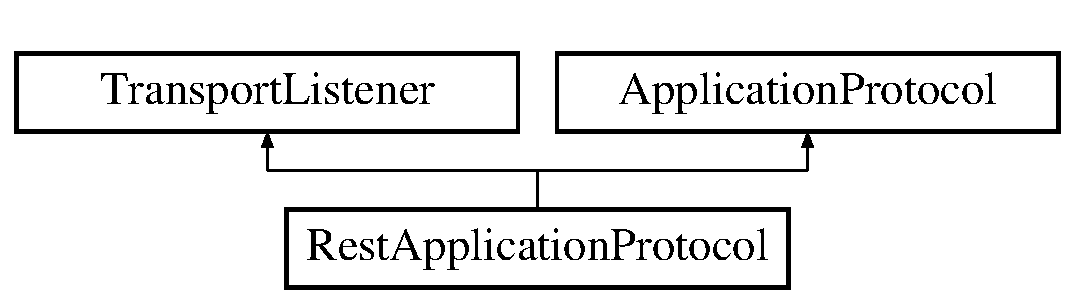
\includegraphics[height=2.000000cm]{class_rest_application_protocol}
\end{center}
\end{figure}
\subsection*{Public Member Functions}
\begin{DoxyCompactItemize}
\item 
\hypertarget{class_rest_application_protocol_a6642fe64e3448d1e524239ab87ff9cfd}{}\hyperlink{class_rest_application_protocol_a6642fe64e3448d1e524239ab87ff9cfd}{Rest\+Application\+Protocol} (\hyperlink{class_transport_protocol}{Transport\+Protocol} \&t)\label{class_rest_application_protocol_a6642fe64e3448d1e524239ab87ff9cfd}

\begin{DoxyCompactList}\small\item\em Second constructor with support for the \hyperlink{class_transport_protocol}{Transport\+Protocol}. \end{DoxyCompactList}\item 
\hypertarget{class_rest_application_protocol_a869529fb061e565fedfe556bc0b13962}{}\hyperlink{class_rest_application_protocol_a869529fb061e565fedfe556bc0b13962}{$\sim$\+Rest\+Application\+Protocol} ()\label{class_rest_application_protocol_a869529fb061e565fedfe556bc0b13962}

\begin{DoxyCompactList}\small\item\em Destructs the \hyperlink{class_application_protocol}{Application\+Protocol} object so the \hyperlink{class_transport_protocol}{Transport\+Protocol} is also removed. \end{DoxyCompactList}\item 
void \hyperlink{class_rest_application_protocol_a1df053880d539be48c83693739bb033e}{add\+Callback\+Function} (std\+::string link, std\+::string method, R\+E\+S\+T\+Call\+Back $\ast$callback\+\_\+addition)
\item 
void \hyperlink{class_rest_application_protocol_a79abf85e9dc1b650ab059735237fde8e}{data\+\_\+received} (uint8\+\_\+t $\ast$data, int number\+\_\+of\+\_\+bytes) override
\item 
void \hyperlink{class_rest_application_protocol_aef36c940842a56d6e8ca520f3c648852}{invoke\+Api\+Call} (std\+::string link, std\+::string method, std\+::string message)
\item 
void \hyperlink{class_rest_application_protocol_a4a979770d89ba354d8321c2d4c751e05}{get\+Json\+A\+P\+I\+Dump} (std\+::string file\+\_\+name)
\end{DoxyCompactItemize}
\subsection*{Additional Inherited Members}


\subsection{Detailed Description}
An extension on \hyperlink{class_application_protocol}{Application\+Protocol} with support for R\+E\+S\+T api. \begin{DoxyAuthor}{Author}
Koen van der Kruk 
\end{DoxyAuthor}
\begin{DoxyVersion}{Version}
1.\+0 
\end{DoxyVersion}
\begin{DoxyDate}{Date}
8-\/6-\/2016 
\end{DoxyDate}


\subsection{Member Function Documentation}
\hypertarget{class_rest_application_protocol_a1df053880d539be48c83693739bb033e}{}\index{Rest\+Application\+Protocol@{Rest\+Application\+Protocol}!add\+Callback\+Function@{add\+Callback\+Function}}
\index{add\+Callback\+Function@{add\+Callback\+Function}!Rest\+Application\+Protocol@{Rest\+Application\+Protocol}}
\subsubsection[{add\+Callback\+Function}]{\setlength{\rightskip}{0pt plus 5cm}void Rest\+Application\+Protocol\+::add\+Callback\+Function (
\begin{DoxyParamCaption}
\item[{std\+::string}]{link, }
\item[{std\+::string}]{method, }
\item[{R\+E\+S\+T\+Call\+Back $\ast$}]{callback\+\_\+addition}
\end{DoxyParamCaption}
)}\label{class_rest_application_protocol_a1df053880d539be48c83693739bb033e}
This will assign a new function as callback function. 
\begin{DoxyParams}{Parameters}
{\em link} & The http url to access \\
\hline
{\em method} & The http method, such as P\+O\+S\+T, P\+U\+T, D\+E\+L\+E\+T\+E, G\+E\+T \\
\hline
{\em call\+Back\+Addition} & The function that receives the callback message. \\
\hline
\end{DoxyParams}
\hypertarget{class_rest_application_protocol_a79abf85e9dc1b650ab059735237fde8e}{}\index{Rest\+Application\+Protocol@{Rest\+Application\+Protocol}!data\+\_\+received@{data\+\_\+received}}
\index{data\+\_\+received@{data\+\_\+received}!Rest\+Application\+Protocol@{Rest\+Application\+Protocol}}
\subsubsection[{data\+\_\+received}]{\setlength{\rightskip}{0pt plus 5cm}void Rest\+Application\+Protocol\+::data\+\_\+received (
\begin{DoxyParamCaption}
\item[{uint8\+\_\+t $\ast$}]{data, }
\item[{int}]{number\+\_\+of\+\_\+bytes}
\end{DoxyParamCaption}
)\hspace{0.3cm}{\ttfamily [override]}, {\ttfamily [virtual]}}\label{class_rest_application_protocol_a79abf85e9dc1b650ab059735237fde8e}
\hyperlink{class_rest_application_protocol}{Rest\+Application\+Protocol} is a \hyperlink{class_transport_listener}{Transport\+Listener} that will receive incoming messages. 
\begin{DoxyParams}{Parameters}
{\em data} & The incoming data package \\
\hline
\end{DoxyParams}


Implements \hyperlink{class_transport_listener_aafc4dd15ef03baa68b36b45c43c5addd}{Transport\+Listener}.

\hypertarget{class_rest_application_protocol_a4a979770d89ba354d8321c2d4c751e05}{}\index{Rest\+Application\+Protocol@{Rest\+Application\+Protocol}!get\+Json\+A\+P\+I\+Dump@{get\+Json\+A\+P\+I\+Dump}}
\index{get\+Json\+A\+P\+I\+Dump@{get\+Json\+A\+P\+I\+Dump}!Rest\+Application\+Protocol@{Rest\+Application\+Protocol}}
\subsubsection[{get\+Json\+A\+P\+I\+Dump}]{\setlength{\rightskip}{0pt plus 5cm}void Rest\+Application\+Protocol\+::get\+Json\+A\+P\+I\+Dump (
\begin{DoxyParamCaption}
\item[{std\+::string}]{file\+\_\+name}
\end{DoxyParamCaption}
)}\label{class_rest_application_protocol_a4a979770d89ba354d8321c2d4c751e05}
This function will dump a full R\+E\+S\+T api in json format. 
\begin{DoxyParams}{Parameters}
{\em file\+Name} & The filename is used to dump the R\+E\+S\+T A\+P\+I in json format. The same directory is used as the current running program. \\
\hline
\end{DoxyParams}
\hypertarget{class_rest_application_protocol_aef36c940842a56d6e8ca520f3c648852}{}\index{Rest\+Application\+Protocol@{Rest\+Application\+Protocol}!invoke\+Api\+Call@{invoke\+Api\+Call}}
\index{invoke\+Api\+Call@{invoke\+Api\+Call}!Rest\+Application\+Protocol@{Rest\+Application\+Protocol}}
\subsubsection[{invoke\+Api\+Call}]{\setlength{\rightskip}{0pt plus 5cm}void Rest\+Application\+Protocol\+::invoke\+Api\+Call (
\begin{DoxyParamCaption}
\item[{std\+::string}]{link, }
\item[{std\+::string}]{method, }
\item[{std\+::string}]{message}
\end{DoxyParamCaption}
)}\label{class_rest_application_protocol_aef36c940842a56d6e8ca520f3c648852}
Invoke A\+P\+I call, callback to another function. 
\begin{DoxyParams}{Parameters}
{\em link} & The url conencted to the callback function \\
\hline
{\em method} & The H\+T\+T\+P method that can be used to invoke an A\+P\+I call over H\+T\+T\+P. \\
\hline
{\em message} & The message for the callback function \\
\hline
\end{DoxyParams}


The documentation for this class was generated from the following files\+:\begin{DoxyCompactItemize}
\item 
C\+:/\+Users/koen/\+Documents/\+Git\+Hub/communication-\/protocols/source/include/\hyperlink{_rest_application_protocol_8hpp}{Rest\+Application\+Protocol.\+hpp}\item 
C\+:/\+Users/koen/\+Documents/\+Git\+Hub/communication-\/protocols/source/src/Rest\+Application\+Protocol.\+cpp\end{DoxyCompactItemize}

\hypertarget{class_t_c_p_socket}{}\section{T\+C\+P\+Socket Class Reference}
\label{class_t_c_p_socket}\index{T\+C\+P\+Socket@{T\+C\+P\+Socket}}


{\ttfamily \#include $<$T\+C\+P\+Socket.\+hpp$>$}

Inheritance diagram for T\+C\+P\+Socket\+:\begin{figure}[H]
\begin{center}
\leavevmode
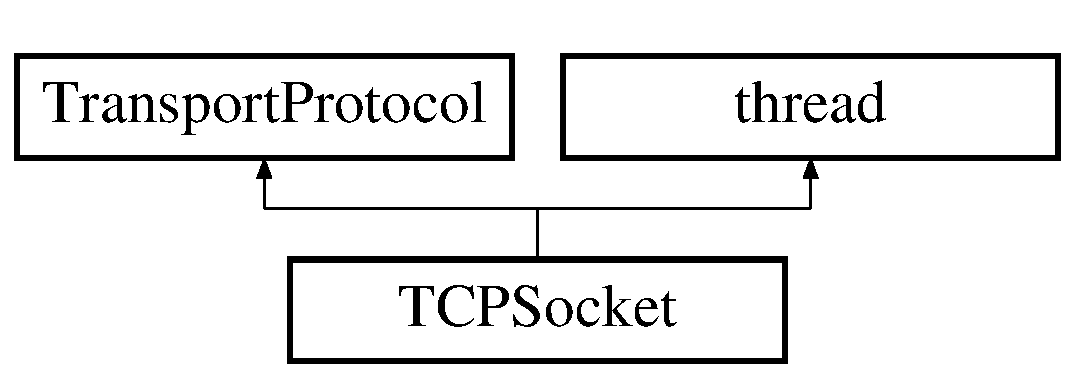
\includegraphics[height=2.000000cm]{class_t_c_p_socket}
\end{center}
\end{figure}
\subsection*{Public Member Functions}
\begin{DoxyCompactItemize}
\item 
\hyperlink{class_t_c_p_socket_ab084bbd93d9b76fd9223f92c12948dde}{T\+C\+P\+Socket} (std\+::string ip\+\_\+nr, std\+::string port\+\_\+nr)
\item 
void \hyperlink{class_t_c_p_socket_ac3622605b73b61ef3c03f49b54036f1e}{init} ()
\item 
void \hyperlink{class_t_c_p_socket_ae083947a4caa02a1a8dd1cc59b2514ac}{data\+\_\+write} (uint8\+\_\+t $\ast$data, int number\+\_\+of\+\_\+bytes) override
\item 
\hypertarget{class_t_c_p_socket_a7ed9a60ec58a60fb132dfa620a4f16a5}{}uint8\+\_\+t $\ast$ \hyperlink{class_t_c_p_socket_a7ed9a60ec58a60fb132dfa620a4f16a5}{data\+\_\+read} () override\label{class_t_c_p_socket_a7ed9a60ec58a60fb132dfa620a4f16a5}

\begin{DoxyCompactList}\small\item\em Reads data from the receive\+\_\+buffer queue. \end{DoxyCompactList}\item 
\hypertarget{class_t_c_p_socket_a66dec2ee5f3a42c066612dcc9974c7bd}{}void \hyperlink{class_t_c_p_socket_a66dec2ee5f3a42c066612dcc9974c7bd}{connect} () override\label{class_t_c_p_socket_a66dec2ee5f3a42c066612dcc9974c7bd}

\begin{DoxyCompactList}\small\item\em Establisching the T\+C\+P connection. \end{DoxyCompactList}\item 
\hypertarget{class_t_c_p_socket_a0d5643435da61bb4a247240e349ac294}{}void \hyperlink{class_t_c_p_socket_a0d5643435da61bb4a247240e349ac294}{disconnect} () override\label{class_t_c_p_socket_a0d5643435da61bb4a247240e349ac294}

\begin{DoxyCompactList}\small\item\em Disconnet the T\+C\+P connection. \end{DoxyCompactList}\item 
\hypertarget{class_t_c_p_socket_a6d0240e24c16c9df20bb0d848e514ae9}{}void \hyperlink{class_t_c_p_socket_a6d0240e24c16c9df20bb0d848e514ae9}{flush} () override\label{class_t_c_p_socket_a6d0240e24c16c9df20bb0d848e514ae9}

\begin{DoxyCompactList}\small\item\em Flushes the send\+\_\+buffer \& receive\+\_\+buffer . \end{DoxyCompactList}\item 
\hypertarget{class_t_c_p_socket_a1cce60b6b2d343bb13692d313c23330f}{}bool \hyperlink{class_t_c_p_socket_a1cce60b6b2d343bb13692d313c23330f}{is\+\_\+open} () override\label{class_t_c_p_socket_a1cce60b6b2d343bb13692d313c23330f}

\begin{DoxyCompactList}\small\item\em Method for checking if the connection is established. \end{DoxyCompactList}\item 
void \hyperlink{class_t_c_p_socket_ab3821e52ca9e792223d9dbc1c45f722f}{send\+\_\+message} ()
\item 
\hypertarget{class_t_c_p_socket_af9110e6f5eb1a535b0b1d4c4ddf20c85}{}void \hyperlink{class_t_c_p_socket_af9110e6f5eb1a535b0b1d4c4ddf20c85}{send\+\_\+message} (uint8\+\_\+t $\ast$d)\label{class_t_c_p_socket_af9110e6f5eb1a535b0b1d4c4ddf20c85}

\begin{DoxyCompactList}\small\item\em Sends the given message to the connected T\+C\+P connection. \end{DoxyCompactList}\item 
void \hyperlink{class_t_c_p_socket_aacbd74adbc7c55fa4176c76021a043e7}{receive\+\_\+message} ()
\item 
\hypertarget{class_t_c_p_socket_a33138c2dbceb68dcc417e8c81ba35188}{}void \hyperlink{class_t_c_p_socket_a33138c2dbceb68dcc417e8c81ba35188}{set\+\_\+receive\+\_\+timeout} (unsigned int i)\label{class_t_c_p_socket_a33138c2dbceb68dcc417e8c81ba35188}

\begin{DoxyCompactList}\small\item\em Sets the timeout for. \end{DoxyCompactList}\item 
void \hyperlink{class_t_c_p_socket_a074a08d48b3ec4e758f0d5fc287a32c2}{set\+\_\+listener} (\hyperlink{class_transport_listener}{Transport\+Listener} $\ast$t) override
\item 
void \hyperlink{class_t_c_p_socket_ab7bce90af0f70773836fab6b7edc6fbd}{remove\+\_\+listener} (\hyperlink{class_transport_listener}{Transport\+Listener} $\ast$t) override
\item 
void \hyperlink{class_t_c_p_socket_adfe57d4441473459b2150556fd6f421b}{run} ()
\end{DoxyCompactItemize}
\subsection*{Additional Inherited Members}


\subsection{Detailed Description}
A protocol class for \hyperlink{class_t_c_p_socket}{T\+C\+P\+Socket}, wrapper for the winsock library. \begin{DoxyAuthor}{Author}
Waila Woe 
\end{DoxyAuthor}
\begin{DoxyVersion}{Version}
1.\+0 
\end{DoxyVersion}
\begin{DoxyDate}{Date}
13-\/6-\/2016 
\end{DoxyDate}


\subsection{Constructor \& Destructor Documentation}
\hypertarget{class_t_c_p_socket_ab084bbd93d9b76fd9223f92c12948dde}{}\index{T\+C\+P\+Socket@{T\+C\+P\+Socket}!T\+C\+P\+Socket@{T\+C\+P\+Socket}}
\index{T\+C\+P\+Socket@{T\+C\+P\+Socket}!T\+C\+P\+Socket@{T\+C\+P\+Socket}}
\subsubsection[{T\+C\+P\+Socket}]{\setlength{\rightskip}{0pt plus 5cm}T\+C\+P\+Socket\+::\+T\+C\+P\+Socket (
\begin{DoxyParamCaption}
\item[{std\+::string}]{ip\+\_\+nr, }
\item[{std\+::string}]{port\+\_\+nr}
\end{DoxyParamCaption}
)}\label{class_t_c_p_socket_ab084bbd93d9b76fd9223f92c12948dde}
The constructor for T\+C\+P 
\begin{DoxyParams}{Parameters}
{\em ip\+Nr} & The ip addres you want to connect to \\
\hline
{\em port\+N\+R} & The port number which it will be connected to \\
\hline
\end{DoxyParams}


\subsection{Member Function Documentation}
\hypertarget{class_t_c_p_socket_ae083947a4caa02a1a8dd1cc59b2514ac}{}\index{T\+C\+P\+Socket@{T\+C\+P\+Socket}!data\+\_\+write@{data\+\_\+write}}
\index{data\+\_\+write@{data\+\_\+write}!T\+C\+P\+Socket@{T\+C\+P\+Socket}}
\subsubsection[{data\+\_\+write}]{\setlength{\rightskip}{0pt plus 5cm}void T\+C\+P\+Socket\+::data\+\_\+write (
\begin{DoxyParamCaption}
\item[{uint8\+\_\+t $\ast$}]{data, }
\item[{int}]{number\+\_\+of\+\_\+bytes}
\end{DoxyParamCaption}
)\hspace{0.3cm}{\ttfamily [override]}, {\ttfamily [virtual]}}\label{class_t_c_p_socket_ae083947a4caa02a1a8dd1cc59b2514ac}
Writes data to the send\+\_\+buffer queue. 
\begin{DoxyParams}{Parameters}
{\em data} & The data to be send. \\
\hline
{\em number\+Of\+Bytes} & Number of bytes that data contains. \\
\hline
\end{DoxyParams}


Implements \hyperlink{class_transport_protocol_af3f6c35f652d73ea3170c64d2b96ff53}{Transport\+Protocol}.

\hypertarget{class_t_c_p_socket_ac3622605b73b61ef3c03f49b54036f1e}{}\index{T\+C\+P\+Socket@{T\+C\+P\+Socket}!init@{init}}
\index{init@{init}!T\+C\+P\+Socket@{T\+C\+P\+Socket}}
\subsubsection[{init}]{\setlength{\rightskip}{0pt plus 5cm}void T\+C\+P\+Socket\+::init (
\begin{DoxyParamCaption}
{}
\end{DoxyParamCaption}
)}\label{class_t_c_p_socket_ac3622605b73b61ef3c03f49b54036f1e}
Initialize winsock Will be called in the constructor to initialize winsock. Do not change this. \hypertarget{class_t_c_p_socket_aacbd74adbc7c55fa4176c76021a043e7}{}\index{T\+C\+P\+Socket@{T\+C\+P\+Socket}!receive\+\_\+message@{receive\+\_\+message}}
\index{receive\+\_\+message@{receive\+\_\+message}!T\+C\+P\+Socket@{T\+C\+P\+Socket}}
\subsubsection[{receive\+\_\+message}]{\setlength{\rightskip}{0pt plus 5cm}void T\+C\+P\+Socket\+::receive\+\_\+message (
\begin{DoxyParamCaption}
{}
\end{DoxyParamCaption}
)}\label{class_t_c_p_socket_aacbd74adbc7c55fa4176c76021a043e7}
Waits untill data is received from the sender and puts the received data in the receive\+\_\+buffer queue. \hypertarget{class_t_c_p_socket_ab7bce90af0f70773836fab6b7edc6fbd}{}\index{T\+C\+P\+Socket@{T\+C\+P\+Socket}!remove\+\_\+listener@{remove\+\_\+listener}}
\index{remove\+\_\+listener@{remove\+\_\+listener}!T\+C\+P\+Socket@{T\+C\+P\+Socket}}
\subsubsection[{remove\+\_\+listener}]{\setlength{\rightskip}{0pt plus 5cm}void T\+C\+P\+Socket\+::remove\+\_\+listener (
\begin{DoxyParamCaption}
\item[{{\bf Transport\+Listener} $\ast$}]{t}
\end{DoxyParamCaption}
)\hspace{0.3cm}{\ttfamily [override]}, {\ttfamily [virtual]}}\label{class_t_c_p_socket_ab7bce90af0f70773836fab6b7edc6fbd}
Method for removing a listener to the listeners list. 
\begin{DoxyParams}{Parameters}
{\em t} & \hyperlink{class_transport_listener}{Transport\+Listener} to be removed \\
\hline
\end{DoxyParams}


Implements \hyperlink{class_transport_protocol_ac7fcdf3b49efae156223bb3351c49553}{Transport\+Protocol}.

\hypertarget{class_t_c_p_socket_adfe57d4441473459b2150556fd6f421b}{}\index{T\+C\+P\+Socket@{T\+C\+P\+Socket}!run@{run}}
\index{run@{run}!T\+C\+P\+Socket@{T\+C\+P\+Socket}}
\subsubsection[{run}]{\setlength{\rightskip}{0pt plus 5cm}void T\+C\+P\+Socket\+::run (
\begin{DoxyParamCaption}
{}
\end{DoxyParamCaption}
)}\label{class_t_c_p_socket_adfe57d4441473459b2150556fd6f421b}
Active method which should run in it\textquotesingle{}s own thread. Sends data in the send\+\_\+buffer through the established connection, and polls for received data while putting it in the receive\+\_\+buffer. \hypertarget{class_t_c_p_socket_ab3821e52ca9e792223d9dbc1c45f722f}{}\index{T\+C\+P\+Socket@{T\+C\+P\+Socket}!send\+\_\+message@{send\+\_\+message}}
\index{send\+\_\+message@{send\+\_\+message}!T\+C\+P\+Socket@{T\+C\+P\+Socket}}
\subsubsection[{send\+\_\+message}]{\setlength{\rightskip}{0pt plus 5cm}void T\+C\+P\+Socket\+::send\+\_\+message (
\begin{DoxyParamCaption}
{}
\end{DoxyParamCaption}
)}\label{class_t_c_p_socket_ab3821e52ca9e792223d9dbc1c45f722f}
Checks for messages in the send\+\_\+buffer queue to send to the connected T\+C\+P Connection. \hypertarget{class_t_c_p_socket_a074a08d48b3ec4e758f0d5fc287a32c2}{}\index{T\+C\+P\+Socket@{T\+C\+P\+Socket}!set\+\_\+listener@{set\+\_\+listener}}
\index{set\+\_\+listener@{set\+\_\+listener}!T\+C\+P\+Socket@{T\+C\+P\+Socket}}
\subsubsection[{set\+\_\+listener}]{\setlength{\rightskip}{0pt plus 5cm}void T\+C\+P\+Socket\+::set\+\_\+listener (
\begin{DoxyParamCaption}
\item[{{\bf Transport\+Listener} $\ast$}]{t}
\end{DoxyParamCaption}
)\hspace{0.3cm}{\ttfamily [override]}, {\ttfamily [virtual]}}\label{class_t_c_p_socket_a074a08d48b3ec4e758f0d5fc287a32c2}
Method for adding a listener to the listeners list. 
\begin{DoxyParams}{Parameters}
{\em t} & \hyperlink{class_transport_listener}{Transport\+Listener} to be added \\
\hline
\end{DoxyParams}


Implements \hyperlink{class_transport_protocol_ad7a9c131bbd9b2a26f1884b18ce11820}{Transport\+Protocol}.



The documentation for this class was generated from the following files\+:\begin{DoxyCompactItemize}
\item 
C\+:/\+Users/koen/\+Documents/\+Git\+Hub/communication-\/protocols/source/include/\hyperlink{_t_c_p_socket_8hpp}{T\+C\+P\+Socket.\+hpp}\item 
C\+:/\+Users/koen/\+Documents/\+Git\+Hub/communication-\/protocols/source/src/T\+C\+P\+Socket.\+cpp\end{DoxyCompactItemize}

\hypertarget{class_transport_listener}{}\section{Transport\+Listener Class Reference}
\label{class_transport_listener}\index{Transport\+Listener@{Transport\+Listener}}


{\ttfamily \#include $<$Transport\+Listener.\+hpp$>$}

Inheritance diagram for Transport\+Listener\+:\begin{figure}[H]
\begin{center}
\leavevmode
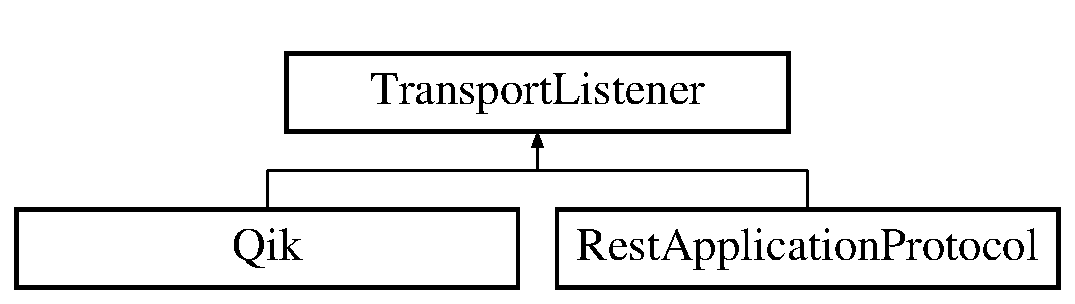
\includegraphics[height=2.000000cm]{class_transport_listener}
\end{center}
\end{figure}
\subsection*{Public Member Functions}
\begin{DoxyCompactItemize}
\item 
virtual void \hyperlink{class_transport_listener_aafc4dd15ef03baa68b36b45c43c5addd}{data\+\_\+received} (uint8\+\_\+t $\ast$data, int number\+\_\+of\+\_\+bytes)=0
\end{DoxyCompactItemize}


\subsection{Detailed Description}
A listener interface to comminucatie to R\+E\+S\+T application protocol. This can be used for protocols that need T\+C\+P access. \begin{DoxyAuthor}{Author}
Koen van der Kruk 
\end{DoxyAuthor}
\begin{DoxyVersion}{Version}
1.\+0 
\end{DoxyVersion}
\begin{DoxyDate}{Date}
8-\/6-\/2016 
\end{DoxyDate}


\subsection{Member Function Documentation}
\hypertarget{class_transport_listener_aafc4dd15ef03baa68b36b45c43c5addd}{}\index{Transport\+Listener@{Transport\+Listener}!data\+\_\+received@{data\+\_\+received}}
\index{data\+\_\+received@{data\+\_\+received}!Transport\+Listener@{Transport\+Listener}}
\subsubsection[{data\+\_\+received}]{\setlength{\rightskip}{0pt plus 5cm}virtual void Transport\+Listener\+::data\+\_\+received (
\begin{DoxyParamCaption}
\item[{uint8\+\_\+t $\ast$}]{data, }
\item[{int}]{number\+\_\+of\+\_\+bytes}
\end{DoxyParamCaption}
)\hspace{0.3cm}{\ttfamily [pure virtual]}}\label{class_transport_listener_aafc4dd15ef03baa68b36b45c43c5addd}
This function is called from the \hyperlink{class_transport_protocol}{Transport\+Protocol} to send data between multiple nodes. 
\begin{DoxyParams}{Parameters}
{\em data} & The transfered data to the listener. \\
\hline
\end{DoxyParams}


Implemented in \hyperlink{class_qik_a0104c2a0c22fbbf83de456cc7cb9840d}{Qik}, and \hyperlink{class_rest_application_protocol_a79abf85e9dc1b650ab059735237fde8e}{Rest\+Application\+Protocol}.



The documentation for this class was generated from the following file\+:\begin{DoxyCompactItemize}
\item 
C\+:/\+Users/koen/\+Documents/\+Git\+Hub/communication-\/protocols/source/include/\hyperlink{_transport_listener_8hpp}{Transport\+Listener.\+hpp}\end{DoxyCompactItemize}

\hypertarget{class_transport_protocol}{}\section{Transport\+Protocol Class Reference}
\label{class_transport_protocol}\index{Transport\+Protocol@{Transport\+Protocol}}
Inheritance diagram for Transport\+Protocol\+:\begin{figure}[H]
\begin{center}
\leavevmode
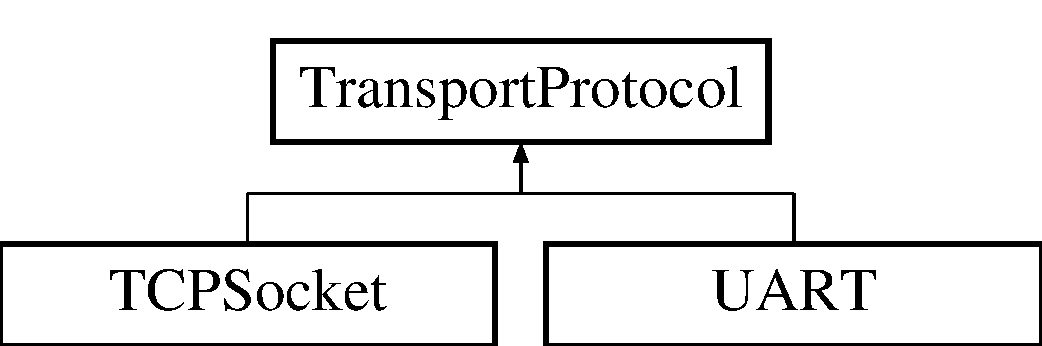
\includegraphics[height=2.000000cm]{class_transport_protocol}
\end{center}
\end{figure}
\subsection*{Public Member Functions}
\begin{DoxyCompactItemize}
\item 
virtual void \hyperlink{class_transport_protocol_af3f6c35f652d73ea3170c64d2b96ff53}{data\+\_\+write} (uint8\+\_\+t $\ast$data, int number\+\_\+of\+\_\+bytes)=0
\item 
\hypertarget{class_transport_protocol_a0145d85c5758e08c94cf60d708eaba08}{}virtual uint8\+\_\+t $\ast$ \hyperlink{class_transport_protocol_a0145d85c5758e08c94cf60d708eaba08}{data\+\_\+read} ()=0\label{class_transport_protocol_a0145d85c5758e08c94cf60d708eaba08}

\begin{DoxyCompactList}\small\item\em Method for reading data from the receive\+\_\+buffer. \end{DoxyCompactList}\item 
\hypertarget{class_transport_protocol_ad0ba1d2982dfaa4b51493548efbf09c6}{}virtual void \hyperlink{class_transport_protocol_ad0ba1d2982dfaa4b51493548efbf09c6}{connect} ()=0\label{class_transport_protocol_ad0ba1d2982dfaa4b51493548efbf09c6}

\begin{DoxyCompactList}\small\item\em Method for establishing the connection. \end{DoxyCompactList}\item 
\hypertarget{class_transport_protocol_a6bc407636830e8e5ff10377b965181eb}{}virtual void \hyperlink{class_transport_protocol_a6bc407636830e8e5ff10377b965181eb}{disconnect} ()=0\label{class_transport_protocol_a6bc407636830e8e5ff10377b965181eb}

\begin{DoxyCompactList}\small\item\em Method for dissolving the connection. \end{DoxyCompactList}\item 
\hypertarget{class_transport_protocol_a1a375d6ab518309c432e56e59043ff4a}{}virtual void \hyperlink{class_transport_protocol_a1a375d6ab518309c432e56e59043ff4a}{flush} ()=0\label{class_transport_protocol_a1a375d6ab518309c432e56e59043ff4a}

\begin{DoxyCompactList}\small\item\em Method for flushing the send\+\_\+buffer and receive\+\_\+buffer. \end{DoxyCompactList}\item 
\hypertarget{class_transport_protocol_aee4e0241f2dbb3cd89712a1e01fe38d4}{}virtual bool \hyperlink{class_transport_protocol_aee4e0241f2dbb3cd89712a1e01fe38d4}{is\+\_\+open} ()=0\label{class_transport_protocol_aee4e0241f2dbb3cd89712a1e01fe38d4}

\begin{DoxyCompactList}\small\item\em Method for checking if the connection is established. \end{DoxyCompactList}\item 
virtual void \hyperlink{class_transport_protocol_ad7a9c131bbd9b2a26f1884b18ce11820}{set\+\_\+listener} (\hyperlink{class_transport_listener}{Transport\+Listener} $\ast$t)=0
\item 
virtual void \hyperlink{class_transport_protocol_ac7fcdf3b49efae156223bb3351c49553}{remove\+\_\+listener} (\hyperlink{class_transport_listener}{Transport\+Listener} $\ast$t)=0
\end{DoxyCompactItemize}
\subsection*{Protected Attributes}
\begin{DoxyCompactItemize}
\item 
\hypertarget{class_transport_protocol_a5b8448f205035c7c89fca15b21009617}{}std\+::vector$<$ \hyperlink{class_transport_listener}{Transport\+Listener} $\ast$ $>$ {\bfseries transport\+\_\+listeners}\label{class_transport_protocol_a5b8448f205035c7c89fca15b21009617}

\item 
\hypertarget{class_transport_protocol_a0319fa0da3f02058ce98e8464f1e119a}{}std\+::queue$<$ uint8\+\_\+t $>$ {\bfseries send\+\_\+buffer}\label{class_transport_protocol_a0319fa0da3f02058ce98e8464f1e119a}

\item 
\hypertarget{class_transport_protocol_a5aa66fcb326af8fce0dfdbad9dfdf675}{}std\+::queue$<$ uint8\+\_\+t $>$ {\bfseries receive\+\_\+buffer}\label{class_transport_protocol_a5aa66fcb326af8fce0dfdbad9dfdf675}

\end{DoxyCompactItemize}


\subsection{Member Function Documentation}
\hypertarget{class_transport_protocol_af3f6c35f652d73ea3170c64d2b96ff53}{}\index{Transport\+Protocol@{Transport\+Protocol}!data\+\_\+write@{data\+\_\+write}}
\index{data\+\_\+write@{data\+\_\+write}!Transport\+Protocol@{Transport\+Protocol}}
\subsubsection[{data\+\_\+write}]{\setlength{\rightskip}{0pt plus 5cm}virtual void Transport\+Protocol\+::data\+\_\+write (
\begin{DoxyParamCaption}
\item[{uint8\+\_\+t $\ast$}]{data, }
\item[{int}]{number\+\_\+of\+\_\+bytes}
\end{DoxyParamCaption}
)\hspace{0.3cm}{\ttfamily [pure virtual]}}\label{class_transport_protocol_af3f6c35f652d73ea3170c64d2b96ff53}
Method for writing data to the send\+\_\+buffer queue, for it to be send through the com port. 
\begin{DoxyParams}{Parameters}
{\em data} & The data to be send \\
\hline
{\em number\+Of\+Bytes} & Length of the data in bytes \\
\hline
\end{DoxyParams}


Implemented in \hyperlink{class_t_c_p_socket_ae083947a4caa02a1a8dd1cc59b2514ac}{T\+C\+P\+Socket}, and \hyperlink{class_u_a_r_t_ad03f74b9d5181ed48aef24a93508c31c}{U\+A\+R\+T}.

\hypertarget{class_transport_protocol_ac7fcdf3b49efae156223bb3351c49553}{}\index{Transport\+Protocol@{Transport\+Protocol}!remove\+\_\+listener@{remove\+\_\+listener}}
\index{remove\+\_\+listener@{remove\+\_\+listener}!Transport\+Protocol@{Transport\+Protocol}}
\subsubsection[{remove\+\_\+listener}]{\setlength{\rightskip}{0pt plus 5cm}virtual void Transport\+Protocol\+::remove\+\_\+listener (
\begin{DoxyParamCaption}
\item[{{\bf Transport\+Listener} $\ast$}]{t}
\end{DoxyParamCaption}
)\hspace{0.3cm}{\ttfamily [pure virtual]}}\label{class_transport_protocol_ac7fcdf3b49efae156223bb3351c49553}
Method for removing a listener to the listeners list. 
\begin{DoxyParams}{Parameters}
{\em t} & \hyperlink{class_transport_listener}{Transport\+Listener} to be removed \\
\hline
\end{DoxyParams}


Implemented in \hyperlink{class_t_c_p_socket_ab7bce90af0f70773836fab6b7edc6fbd}{T\+C\+P\+Socket}, and \hyperlink{class_u_a_r_t_ab70270f949057521043566efbdb7b3c3}{U\+A\+R\+T}.

\hypertarget{class_transport_protocol_ad7a9c131bbd9b2a26f1884b18ce11820}{}\index{Transport\+Protocol@{Transport\+Protocol}!set\+\_\+listener@{set\+\_\+listener}}
\index{set\+\_\+listener@{set\+\_\+listener}!Transport\+Protocol@{Transport\+Protocol}}
\subsubsection[{set\+\_\+listener}]{\setlength{\rightskip}{0pt plus 5cm}virtual void Transport\+Protocol\+::set\+\_\+listener (
\begin{DoxyParamCaption}
\item[{{\bf Transport\+Listener} $\ast$}]{t}
\end{DoxyParamCaption}
)\hspace{0.3cm}{\ttfamily [pure virtual]}}\label{class_transport_protocol_ad7a9c131bbd9b2a26f1884b18ce11820}
Method for adding a listener to the listeners list. 
\begin{DoxyParams}{Parameters}
{\em t} & \hyperlink{class_transport_listener}{Transport\+Listener} to be added \\
\hline
\end{DoxyParams}


Implemented in \hyperlink{class_t_c_p_socket_a074a08d48b3ec4e758f0d5fc287a32c2}{T\+C\+P\+Socket}, and \hyperlink{class_u_a_r_t_a865baf02a528c89bd5c0c2f01e04c2f1}{U\+A\+R\+T}.



The documentation for this class was generated from the following file\+:\begin{DoxyCompactItemize}
\item 
C\+:/\+Users/koen/\+Documents/\+Git\+Hub/communication-\/protocols/source/include/\hyperlink{_transport_protocol_8hpp}{Transport\+Protocol.\+hpp}\end{DoxyCompactItemize}

\hypertarget{class_u_a_r_t}{}\section{U\+A\+R\+T Class Reference}
\label{class_u_a_r_t}\index{U\+A\+R\+T@{U\+A\+R\+T}}


{\ttfamily \#include $<$U\+A\+R\+T.\+hpp$>$}

Inheritance diagram for U\+A\+R\+T\+:\begin{figure}[H]
\begin{center}
\leavevmode
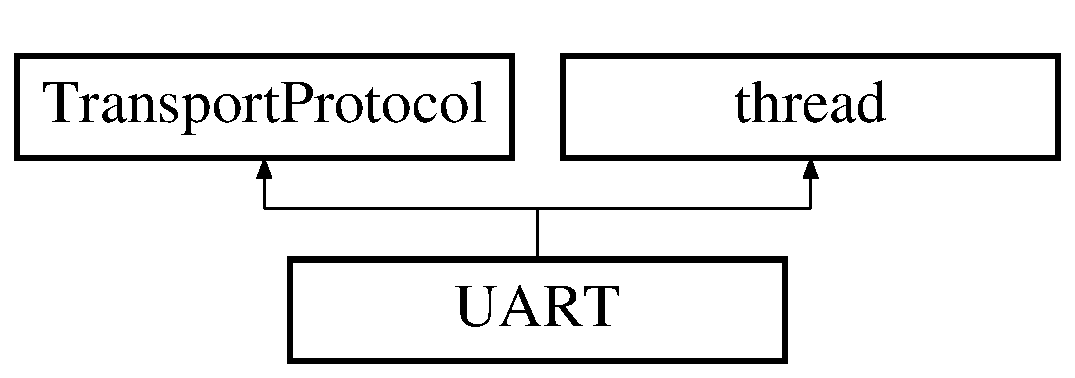
\includegraphics[height=2.000000cm]{class_u_a_r_t}
\end{center}
\end{figure}
\subsection*{Public Member Functions}
\begin{DoxyCompactItemize}
\item 
\hyperlink{class_u_a_r_t_a2912097d50627bf539e3247845ceb899}{U\+A\+R\+T} (int comport\+\_\+nr, int baudrate=9600, const char $\ast$mode=\char`\"{}8\+N1\char`\"{})
\item 
\hypertarget{class_u_a_r_t_a79aea29bd989d2e2ce9692042375b83e}{}\hyperlink{class_u_a_r_t_a79aea29bd989d2e2ce9692042375b83e}{$\sim$\+U\+A\+R\+T} ()\label{class_u_a_r_t_a79aea29bd989d2e2ce9692042375b83e}

\begin{DoxyCompactList}\small\item\em Destructor for \hyperlink{class_u_a_r_t}{U\+A\+R\+T} connection. \end{DoxyCompactList}\item 
void \hyperlink{class_u_a_r_t_ad03f74b9d5181ed48aef24a93508c31c}{data\+\_\+write} (uint8\+\_\+t $\ast$data, int number\+Of\+Bytes) override
\item 
\hypertarget{class_u_a_r_t_a199246f2e9b7d430c30aefd36230321f}{}uint8\+\_\+t $\ast$ \hyperlink{class_u_a_r_t_a199246f2e9b7d430c30aefd36230321f}{data\+\_\+read} () override\label{class_u_a_r_t_a199246f2e9b7d430c30aefd36230321f}

\begin{DoxyCompactList}\small\item\em Method for reading data from the receive\+\_\+buffer. \end{DoxyCompactList}\item 
\hypertarget{class_u_a_r_t_a0ec2cd830665a221b6cd3355cc7ef0e2}{}void \hyperlink{class_u_a_r_t_a0ec2cd830665a221b6cd3355cc7ef0e2}{connect} () override\label{class_u_a_r_t_a0ec2cd830665a221b6cd3355cc7ef0e2}

\begin{DoxyCompactList}\small\item\em Method for establishing the \hyperlink{class_u_a_r_t}{U\+A\+R\+T} connection. \end{DoxyCompactList}\item 
\hypertarget{class_u_a_r_t_a85257ba6ca852314fae7b0c4dd5650c3}{}void \hyperlink{class_u_a_r_t_a85257ba6ca852314fae7b0c4dd5650c3}{disconnect} () override\label{class_u_a_r_t_a85257ba6ca852314fae7b0c4dd5650c3}

\begin{DoxyCompactList}\small\item\em Method for dissolving the \hyperlink{class_u_a_r_t}{U\+A\+R\+T} connection. \end{DoxyCompactList}\item 
void \hyperlink{class_u_a_r_t_ac34a3da482eafe1e32f3b2111a910d2a}{flush} () override
\item 
\hypertarget{class_u_a_r_t_a5551a0313999a799a948b80a407d1e2f}{}bool \hyperlink{class_u_a_r_t_a5551a0313999a799a948b80a407d1e2f}{is\+\_\+open} () override\label{class_u_a_r_t_a5551a0313999a799a948b80a407d1e2f}

\begin{DoxyCompactList}\small\item\em Method for checking if the connection is established. \end{DoxyCompactList}\item 
void \hyperlink{class_u_a_r_t_a865baf02a528c89bd5c0c2f01e04c2f1}{set\+\_\+listener} (\hyperlink{class_transport_listener}{Transport\+Listener} $\ast$t) override
\item 
void \hyperlink{class_u_a_r_t_ab70270f949057521043566efbdb7b3c3}{remove\+\_\+listener} (\hyperlink{class_transport_listener}{Transport\+Listener} $\ast$t) override
\item 
void \hyperlink{class_u_a_r_t_a9efd5e5c4d36ad9f69b9e22feb11ca0e}{run} ()
\end{DoxyCompactItemize}
\subsection*{Additional Inherited Members}


\subsection{Detailed Description}
A protocol class for \hyperlink{class_u_a_r_t}{U\+A\+R\+T}, wrapper for the R\+S232 library. \begin{DoxyAuthor}{Author}
Thijs Hendrickx 
\end{DoxyAuthor}
\begin{DoxyVersion}{Version}
1.\+0 
\end{DoxyVersion}
\begin{DoxyDate}{Date}
13-\/6-\/2016 
\end{DoxyDate}


\subsection{Constructor \& Destructor Documentation}
\hypertarget{class_u_a_r_t_a2912097d50627bf539e3247845ceb899}{}\index{U\+A\+R\+T@{U\+A\+R\+T}!U\+A\+R\+T@{U\+A\+R\+T}}
\index{U\+A\+R\+T@{U\+A\+R\+T}!U\+A\+R\+T@{U\+A\+R\+T}}
\subsubsection[{U\+A\+R\+T}]{\setlength{\rightskip}{0pt plus 5cm}U\+A\+R\+T\+::\+U\+A\+R\+T (
\begin{DoxyParamCaption}
\item[{int}]{comport\+\_\+nr, }
\item[{int}]{baudrate = {\ttfamily 9600}, }
\item[{const char $\ast$}]{mode = {\ttfamily \char`\"{}8N1\char`\"{}}}
\end{DoxyParamCaption}
)}\label{class_u_a_r_t_a2912097d50627bf539e3247845ceb899}
Constructor for initialising \hyperlink{class_u_a_r_t}{U\+A\+R\+T} connection. 
\begin{DoxyParams}{Parameters}
{\em comport\+\_\+nr} & The com port which to connect to. This is for example C\+O\+M4 for windows or tty\+U\+Sb4 for linux. Full list of defines can be found in comport\+\_\+defines.\+hpp \\
\hline
{\em baudrate} & The baudrate to use when sending and receiving data over the selected com port. \\
\hline
{\em mode} & The settings to use for the connection, data bits, parity and stopbits. \\
\hline
\end{DoxyParams}


\subsection{Member Function Documentation}
\hypertarget{class_u_a_r_t_ad03f74b9d5181ed48aef24a93508c31c}{}\index{U\+A\+R\+T@{U\+A\+R\+T}!data\+\_\+write@{data\+\_\+write}}
\index{data\+\_\+write@{data\+\_\+write}!U\+A\+R\+T@{U\+A\+R\+T}}
\subsubsection[{data\+\_\+write}]{\setlength{\rightskip}{0pt plus 5cm}void U\+A\+R\+T\+::data\+\_\+write (
\begin{DoxyParamCaption}
\item[{uint8\+\_\+t $\ast$}]{data, }
\item[{int}]{number\+Of\+Bytes}
\end{DoxyParamCaption}
)\hspace{0.3cm}{\ttfamily [override]}, {\ttfamily [virtual]}}\label{class_u_a_r_t_ad03f74b9d5181ed48aef24a93508c31c}
Method for writing data to the send\+\_\+buffer queue, for it to be send through the com port. 
\begin{DoxyParams}{Parameters}
{\em data} & The data to be send \\
\hline
{\em number\+Of\+Bytes} & Length of the data in bytes \\
\hline
\end{DoxyParams}


Implements \hyperlink{class_transport_protocol_af3f6c35f652d73ea3170c64d2b96ff53}{Transport\+Protocol}.

\hypertarget{class_u_a_r_t_ac34a3da482eafe1e32f3b2111a910d2a}{}\index{U\+A\+R\+T@{U\+A\+R\+T}!flush@{flush}}
\index{flush@{flush}!U\+A\+R\+T@{U\+A\+R\+T}}
\subsubsection[{flush}]{\setlength{\rightskip}{0pt plus 5cm}void U\+A\+R\+T\+::flush (
\begin{DoxyParamCaption}
{}
\end{DoxyParamCaption}
)\hspace{0.3cm}{\ttfamily [override]}, {\ttfamily [virtual]}}\label{class_u_a_r_t_ac34a3da482eafe1e32f3b2111a910d2a}
Method for flushing the send\+\_\+buffer and receive\+\_\+buffer. Also flushes the R\+X and T\+X pins of the com port specified. 

Implements \hyperlink{class_transport_protocol_a1a375d6ab518309c432e56e59043ff4a}{Transport\+Protocol}.

\hypertarget{class_u_a_r_t_ab70270f949057521043566efbdb7b3c3}{}\index{U\+A\+R\+T@{U\+A\+R\+T}!remove\+\_\+listener@{remove\+\_\+listener}}
\index{remove\+\_\+listener@{remove\+\_\+listener}!U\+A\+R\+T@{U\+A\+R\+T}}
\subsubsection[{remove\+\_\+listener}]{\setlength{\rightskip}{0pt plus 5cm}void U\+A\+R\+T\+::remove\+\_\+listener (
\begin{DoxyParamCaption}
\item[{{\bf Transport\+Listener} $\ast$}]{t}
\end{DoxyParamCaption}
)\hspace{0.3cm}{\ttfamily [override]}, {\ttfamily [virtual]}}\label{class_u_a_r_t_ab70270f949057521043566efbdb7b3c3}
Method for removing a listener to the listeners list. 
\begin{DoxyParams}{Parameters}
{\em t} & \hyperlink{class_transport_listener}{Transport\+Listener} to be removed \\
\hline
\end{DoxyParams}


Implements \hyperlink{class_transport_protocol_ac7fcdf3b49efae156223bb3351c49553}{Transport\+Protocol}.

\hypertarget{class_u_a_r_t_a9efd5e5c4d36ad9f69b9e22feb11ca0e}{}\index{U\+A\+R\+T@{U\+A\+R\+T}!run@{run}}
\index{run@{run}!U\+A\+R\+T@{U\+A\+R\+T}}
\subsubsection[{run}]{\setlength{\rightskip}{0pt plus 5cm}void U\+A\+R\+T\+::run (
\begin{DoxyParamCaption}
{}
\end{DoxyParamCaption}
)}\label{class_u_a_r_t_a9efd5e5c4d36ad9f69b9e22feb11ca0e}
Active method which should run in it\textquotesingle{}s own thread. Sends data in the send\+\_\+buffer through the established connection, and polls the com port for received data while putting it in the receive\+\_\+buffer. \hypertarget{class_u_a_r_t_a865baf02a528c89bd5c0c2f01e04c2f1}{}\index{U\+A\+R\+T@{U\+A\+R\+T}!set\+\_\+listener@{set\+\_\+listener}}
\index{set\+\_\+listener@{set\+\_\+listener}!U\+A\+R\+T@{U\+A\+R\+T}}
\subsubsection[{set\+\_\+listener}]{\setlength{\rightskip}{0pt plus 5cm}void U\+A\+R\+T\+::set\+\_\+listener (
\begin{DoxyParamCaption}
\item[{{\bf Transport\+Listener} $\ast$}]{t}
\end{DoxyParamCaption}
)\hspace{0.3cm}{\ttfamily [override]}, {\ttfamily [virtual]}}\label{class_u_a_r_t_a865baf02a528c89bd5c0c2f01e04c2f1}
Method for adding a listener to the listeners list. 
\begin{DoxyParams}{Parameters}
{\em t} & \hyperlink{class_transport_listener}{Transport\+Listener} to be added \\
\hline
\end{DoxyParams}


Implements \hyperlink{class_transport_protocol_ad7a9c131bbd9b2a26f1884b18ce11820}{Transport\+Protocol}.



The documentation for this class was generated from the following files\+:\begin{DoxyCompactItemize}
\item 
C\+:/\+Users/koen/\+Documents/\+Git\+Hub/communication-\/protocols/source/include/\hyperlink{_u_a_r_t_8hpp}{U\+A\+R\+T.\+hpp}\item 
C\+:/\+Users/koen/\+Documents/\+Git\+Hub/communication-\/protocols/source/src/U\+A\+R\+T.\+cpp\end{DoxyCompactItemize}

\chapter{File Documentation}
\hypertarget{_application_protocol_8hpp}{}\section{C\+:/\+Users/koen/\+Documents/\+Git\+Hub/communication-\/protocols/source/include/\+Application\+Protocol.hpp File Reference}
\label{_application_protocol_8hpp}\index{C\+:/\+Users/koen/\+Documents/\+Git\+Hub/communication-\/protocols/source/include/\+Application\+Protocol.\+hpp@{C\+:/\+Users/koen/\+Documents/\+Git\+Hub/communication-\/protocols/source/include/\+Application\+Protocol.\+hpp}}


\hyperlink{class_application_protocol}{Application\+Protocol} is used to define a type that other applications can use. Such as \hyperlink{class_qik}{Qik} and R\+E\+S\+T.  


{\ttfamily \#include \char`\"{}Transport\+Protocol.\+hpp\char`\"{}}\\*
\subsection*{Classes}
\begin{DoxyCompactItemize}
\item 
class \hyperlink{class_application_protocol}{Application\+Protocol}
\end{DoxyCompactItemize}


\subsection{Detailed Description}
\hyperlink{class_application_protocol}{Application\+Protocol} is used to define a type that other applications can use. Such as \hyperlink{class_qik}{Qik} and R\+E\+S\+T. 

\begin{DoxyAuthor}{Author}
Koen van der Kruk, 1654581 
\end{DoxyAuthor}
\begin{DoxyDate}{Date}
Created\+: 16-\/6-\/2016 

Last Modified\+: 16-\/6-\/2016 \hyperlink{class_application_protocol}{Application\+Protocol} is used to define one way to talk to other applications with a \hyperlink{class_transport_protocol}{Transport\+Protocol}
\end{DoxyDate}
\begin{DoxyCopyright}{Copyright}
Copyright © 2016, H\+U University of Applied Sciences Utrecht. All rights reserved.
\end{DoxyCopyright}
License\+: new\+B\+S\+D

Redistribution and use in source and binary forms, with or without modification, are permitted provided that the following conditions are met\+:
\begin{DoxyItemize}
\item Redistributions of source code must retain the above copyright notice, this list of conditions and the following disclaimer.
\item Redistributions in binary form must reproduce the above copyright notice, this list of conditions and the following disclaimer in the documentation and/or other materials provided with the distribution.
\item Neither the name of the H\+U University of Applied Sciences Utrecht nor the names of its contributors may be used to endorse or promote products derived from this software without specific prior written permission.
\end{DoxyItemize}

T\+H\+I\+S S\+O\+F\+T\+W\+A\+R\+E I\+S P\+R\+O\+V\+I\+D\+E\+D B\+Y T\+H\+E C\+O\+P\+Y\+R\+I\+G\+H\+T H\+O\+L\+D\+E\+R\+S A\+N\+D C\+O\+N\+T\+R\+I\+B\+U\+T\+O\+R\+S \char`\"{}\+A\+S I\+S\char`\"{} A\+N\+D A\+N\+Y E\+X\+P\+R\+E\+S\+S O\+R I\+M\+P\+L\+I\+E\+D W\+A\+R\+R\+A\+N\+T\+I\+E\+S, I\+N\+C\+L\+U\+D\+I\+N\+G, B\+U\+T N\+O\+T L\+I\+M\+I\+T\+E\+D T\+O, T\+H\+E I\+M\+P\+L\+I\+E\+D W\+A\+R\+R\+A\+N\+T\+I\+E\+S O\+F M\+E\+R\+C\+H\+A\+N\+T\+A\+B\+I\+L\+I\+T\+Y A\+N\+D F\+I\+T\+N\+E\+S\+S F\+O\+R A P\+A\+R\+T\+I\+C\+U\+L\+A\+R P\+U\+R\+P\+O\+S\+E A\+R\+E D\+I\+S\+C\+L\+A\+I\+M\+E\+D. I\+N N\+O E\+V\+E\+N\+T S\+H\+A\+L\+L T\+H\+E H\+U U\+N\+I\+V\+E\+R\+S\+I\+T\+Y O\+F A\+P\+P\+L\+I\+E\+D S\+C\+I\+E\+N\+C\+E\+S U\+T\+R\+E\+C\+H\+T B\+E L\+I\+A\+B\+L\+E F\+O\+R A\+N\+Y D\+I\+R\+E\+C\+T, I\+N\+D\+I\+R\+E\+C\+T, I\+N\+C\+I\+D\+E\+N\+T\+A\+L, S\+P\+E\+C\+I\+A\+L, E\+X\+E\+M\+P\+L\+A\+R\+Y, O\+R C\+O\+N\+S\+E\+Q\+U\+E\+N\+T\+I\+A\+L D\+A\+M\+A\+G\+E\+S (I\+N\+C\+L\+U\+D\+I\+N\+G, B\+U\+T N\+O\+T L\+I\+M\+I\+T\+E\+D T\+O, P\+R\+O\+C\+U\+R\+E\+M\+E\+N\+T O\+F S\+U\+B\+S\+T\+I\+T\+U\+T\+E G\+O\+O\+D\+S O\+R S\+E\+R\+V\+I\+C\+E\+S; L\+O\+S\+S O\+F U\+S\+E, D\+A\+T\+A, O\+R P\+R\+O\+F\+I\+T\+S; O\+R B\+U\+S\+I\+N\+E\+S\+S I\+N\+T\+E\+R\+R\+U\+P\+T\+I\+O\+N) H\+O\+W\+E\+V\+E\+R C\+A\+U\+S\+E\+D A\+N\+D O\+N A\+N\+Y T\+H\+E\+O\+R\+Y O\+F L\+I\+A\+B\+I\+L\+I\+T\+Y, W\+H\+E\+T\+H\+E\+R I\+N C\+O\+N\+T\+R\+A\+C\+T, S\+T\+R\+I\+C\+T L\+I\+A\+B\+I\+L\+I\+T\+Y, O\+R T\+O\+R\+T (I\+N\+C\+L\+U\+D\+I\+N\+G N\+E\+G\+L\+I\+G\+E\+N\+C\+E O\+R O\+T\+H\+E\+R\+W\+I\+S\+E) A\+R\+I\+S\+I\+N\+G I\+N A\+N\+Y W\+A\+Y O\+U\+T O\+F T\+H\+E U\+S\+E O\+F T\+H\+I\+S S\+O\+F\+T\+W\+A\+R\+E, E\+V\+E\+N I\+F A\+D\+V\+I\+S\+E\+D O\+F T\+H\+E P\+O\+S\+S\+I\+B\+I\+L\+I\+T\+Y O\+F S\+U\+C\+H D\+A\+M\+A\+G\+E. 
\hypertarget{_comport_defines_8hpp}{}\section{C\+:/\+Users/koen/\+Documents/\+Git\+Hub/communication-\/protocols/source/include/\+Comport\+Defines.hpp File Reference}
\label{_comport_defines_8hpp}\index{C\+:/\+Users/koen/\+Documents/\+Git\+Hub/communication-\/protocols/source/include/\+Comport\+Defines.\+hpp@{C\+:/\+Users/koen/\+Documents/\+Git\+Hub/communication-\/protocols/source/include/\+Comport\+Defines.\+hpp}}


Comport\+Defines is used to define all the different comports in a cygwin (windows) system.  


\subsection*{Variables}
\begin{DoxyCompactItemize}
\item 
\hypertarget{_comport_defines_8hpp_ae93bba0243a5c05835e663b6ac631da5}{}constexpr int {\bfseries tty\+S0} = 0\label{_comport_defines_8hpp_ae93bba0243a5c05835e663b6ac631da5}

\item 
\hypertarget{_comport_defines_8hpp_a07b28451273cdc798d546cc700ef660d}{}constexpr int {\bfseries C\+O\+M1} = 0\label{_comport_defines_8hpp_a07b28451273cdc798d546cc700ef660d}

\item 
\hypertarget{_comport_defines_8hpp_a3a6fbdb6687c566fb589daf9d38b1a4f}{}constexpr int {\bfseries tty\+S1} = 1\label{_comport_defines_8hpp_a3a6fbdb6687c566fb589daf9d38b1a4f}

\item 
\hypertarget{_comport_defines_8hpp_a3ca0f48cac28c4ffd19f35b850995ab9}{}constexpr int {\bfseries C\+O\+M2} = 1\label{_comport_defines_8hpp_a3ca0f48cac28c4ffd19f35b850995ab9}

\item 
\hypertarget{_comport_defines_8hpp_a07dd4414a36ce78a6edb81855561666b}{}constexpr int {\bfseries tty\+S2} = 2\label{_comport_defines_8hpp_a07dd4414a36ce78a6edb81855561666b}

\item 
\hypertarget{_comport_defines_8hpp_ad9f1b55e8ea933a2c14c8c588ccabce9}{}constexpr int {\bfseries C\+O\+M3} = 2\label{_comport_defines_8hpp_ad9f1b55e8ea933a2c14c8c588ccabce9}

\item 
\hypertarget{_comport_defines_8hpp_afdb05fc55d52f119d460b3bf64299292}{}constexpr int {\bfseries tty\+S3} = 3\label{_comport_defines_8hpp_afdb05fc55d52f119d460b3bf64299292}

\item 
\hypertarget{_comport_defines_8hpp_a374c39ca15b2fe2b9294cda63b335a30}{}constexpr int {\bfseries C\+O\+M4} = 3\label{_comport_defines_8hpp_a374c39ca15b2fe2b9294cda63b335a30}

\item 
\hypertarget{_comport_defines_8hpp_a01ae74cd4cf9e232e0a2b497b6ebc8f3}{}constexpr int {\bfseries tty\+S4} = 4\label{_comport_defines_8hpp_a01ae74cd4cf9e232e0a2b497b6ebc8f3}

\item 
\hypertarget{_comport_defines_8hpp_a4b1c3e1c3f1fe553c81d64218aae4d75}{}constexpr int {\bfseries C\+O\+M5} = 4\label{_comport_defines_8hpp_a4b1c3e1c3f1fe553c81d64218aae4d75}

\item 
\hypertarget{_comport_defines_8hpp_a67c0fe1888aecc45aae0cbc7e8859ffb}{}constexpr int {\bfseries tty\+S5} = 5\label{_comport_defines_8hpp_a67c0fe1888aecc45aae0cbc7e8859ffb}

\item 
\hypertarget{_comport_defines_8hpp_ad8e2a3b26ca45929928a69dfb7c507bb}{}constexpr int {\bfseries C\+O\+M6} = 5\label{_comport_defines_8hpp_ad8e2a3b26ca45929928a69dfb7c507bb}

\item 
\hypertarget{_comport_defines_8hpp_a4e4ff67ff7a6c170113b2f09969f4271}{}constexpr int {\bfseries tty\+S6} = 6\label{_comport_defines_8hpp_a4e4ff67ff7a6c170113b2f09969f4271}

\item 
\hypertarget{_comport_defines_8hpp_a440acacc334f5fa238e1be2ee23fe91a}{}constexpr int {\bfseries C\+O\+M7} = 6\label{_comport_defines_8hpp_a440acacc334f5fa238e1be2ee23fe91a}

\item 
\hypertarget{_comport_defines_8hpp_abeb941742d0252f3c2557a295fec414f}{}constexpr int {\bfseries tty\+S7} = 7\label{_comport_defines_8hpp_abeb941742d0252f3c2557a295fec414f}

\item 
\hypertarget{_comport_defines_8hpp_a0d8d02f59b3bec01936cba3b6900d1d7}{}constexpr int {\bfseries C\+O\+M8} = 7\label{_comport_defines_8hpp_a0d8d02f59b3bec01936cba3b6900d1d7}

\item 
\hypertarget{_comport_defines_8hpp_a902ba21f5aa4b667d7f8d0dafc905d0d}{}constexpr int {\bfseries tty\+S8} = 8\label{_comport_defines_8hpp_a902ba21f5aa4b667d7f8d0dafc905d0d}

\item 
\hypertarget{_comport_defines_8hpp_a1ccb33a10e28e04a241a2a195f907897}{}constexpr int {\bfseries C\+O\+M9} = 8\label{_comport_defines_8hpp_a1ccb33a10e28e04a241a2a195f907897}

\item 
\hypertarget{_comport_defines_8hpp_a2a1aa5357331b2fe63b5e3a59253998c}{}constexpr int {\bfseries tty\+S9} = 9\label{_comport_defines_8hpp_a2a1aa5357331b2fe63b5e3a59253998c}

\item 
\hypertarget{_comport_defines_8hpp_ac36edb9e1df3c55fc4f177f25917f337}{}constexpr int {\bfseries C\+O\+M10} = 9\label{_comport_defines_8hpp_ac36edb9e1df3c55fc4f177f25917f337}

\item 
\hypertarget{_comport_defines_8hpp_a02a84165ddee8d1b189e6f23ba56bd6d}{}constexpr int {\bfseries tty\+S10} = 10\label{_comport_defines_8hpp_a02a84165ddee8d1b189e6f23ba56bd6d}

\item 
\hypertarget{_comport_defines_8hpp_a136b05e8734a7a722654c587c13d5783}{}constexpr int {\bfseries C\+O\+M11} = 10\label{_comport_defines_8hpp_a136b05e8734a7a722654c587c13d5783}

\item 
\hypertarget{_comport_defines_8hpp_a8a6531179cf699e0fa0f96a10accc39f}{}constexpr int {\bfseries tty\+S11} = 11\label{_comport_defines_8hpp_a8a6531179cf699e0fa0f96a10accc39f}

\item 
\hypertarget{_comport_defines_8hpp_a60f237f69bbda3e74492f339ed5f0c7f}{}constexpr int {\bfseries C\+O\+M12} = 11\label{_comport_defines_8hpp_a60f237f69bbda3e74492f339ed5f0c7f}

\item 
\hypertarget{_comport_defines_8hpp_a545b59d57662860ed29e351bad2278ee}{}constexpr int {\bfseries tty\+S12} = 12\label{_comport_defines_8hpp_a545b59d57662860ed29e351bad2278ee}

\item 
\hypertarget{_comport_defines_8hpp_a44f5f54913d342b5c291cab3888ff485}{}constexpr int {\bfseries C\+O\+M13} = 12\label{_comport_defines_8hpp_a44f5f54913d342b5c291cab3888ff485}

\item 
\hypertarget{_comport_defines_8hpp_a76fe884c99cb45504d09efc1546c73a0}{}constexpr int {\bfseries tty\+S13} = 13\label{_comport_defines_8hpp_a76fe884c99cb45504d09efc1546c73a0}

\item 
\hypertarget{_comport_defines_8hpp_ac92bfca9ff8fc5287a1772e4f4745997}{}constexpr int {\bfseries C\+O\+M14} = 13\label{_comport_defines_8hpp_ac92bfca9ff8fc5287a1772e4f4745997}

\item 
\hypertarget{_comport_defines_8hpp_abfdaea1d9954868f5bf64c68ee0c0a8f}{}constexpr int {\bfseries tty\+S14} = 14\label{_comport_defines_8hpp_abfdaea1d9954868f5bf64c68ee0c0a8f}

\item 
\hypertarget{_comport_defines_8hpp_af1f6a04337de5752d77ed156c9f29ec5}{}constexpr int {\bfseries C\+O\+M15} = 14\label{_comport_defines_8hpp_af1f6a04337de5752d77ed156c9f29ec5}

\item 
\hypertarget{_comport_defines_8hpp_aa5f3a885330eda268418ec65339c9995}{}constexpr int {\bfseries tty\+S15} = 15\label{_comport_defines_8hpp_aa5f3a885330eda268418ec65339c9995}

\item 
\hypertarget{_comport_defines_8hpp_a1720ebee948e53346a6874bacf94daa5}{}constexpr int {\bfseries C\+O\+M16} = 15\label{_comport_defines_8hpp_a1720ebee948e53346a6874bacf94daa5}

\item 
\hypertarget{_comport_defines_8hpp_accfa350342c0ad29181ec495d9e2fda4}{}constexpr int {\bfseries tty\+U\+S\+B0} = 16\label{_comport_defines_8hpp_accfa350342c0ad29181ec495d9e2fda4}

\item 
\hypertarget{_comport_defines_8hpp_a75c17e856f33f59d7f7acbe3b36a370b}{}constexpr int {\bfseries tty\+U\+S\+B1} = 17\label{_comport_defines_8hpp_a75c17e856f33f59d7f7acbe3b36a370b}

\item 
\hypertarget{_comport_defines_8hpp_a2e78d64f31b9e14c8dad8866532e84b6}{}constexpr int {\bfseries tty\+U\+S\+B2} = 18\label{_comport_defines_8hpp_a2e78d64f31b9e14c8dad8866532e84b6}

\item 
\hypertarget{_comport_defines_8hpp_a81a7537c578292bbbec7b90f961c0f17}{}constexpr int {\bfseries tty\+U\+S\+B3} = 19\label{_comport_defines_8hpp_a81a7537c578292bbbec7b90f961c0f17}

\item 
\hypertarget{_comport_defines_8hpp_a8650bcd2b34f2efdaff4d6891ab9807d}{}constexpr int {\bfseries tty\+U\+S\+B4} = 20\label{_comport_defines_8hpp_a8650bcd2b34f2efdaff4d6891ab9807d}

\item 
\hypertarget{_comport_defines_8hpp_ad59fb68e176eed81a4402dd5e52d0af7}{}constexpr int {\bfseries tty\+U\+S\+B5} = 21\label{_comport_defines_8hpp_ad59fb68e176eed81a4402dd5e52d0af7}

\item 
\hypertarget{_comport_defines_8hpp_a3629c7b1ad387564ef0798c8235e4b52}{}constexpr int {\bfseries tty\+A\+M\+A0} = 22\label{_comport_defines_8hpp_a3629c7b1ad387564ef0798c8235e4b52}

\item 
\hypertarget{_comport_defines_8hpp_a793a7595c593a92a6cff616faa6b28ed}{}constexpr int {\bfseries tty\+A\+M\+A1} = 23\label{_comport_defines_8hpp_a793a7595c593a92a6cff616faa6b28ed}

\item 
\hypertarget{_comport_defines_8hpp_a60ee4280ec91df19af931e1f03bbf081}{}constexpr int {\bfseries tty\+A\+C\+M0} = 24\label{_comport_defines_8hpp_a60ee4280ec91df19af931e1f03bbf081}

\item 
\hypertarget{_comport_defines_8hpp_a4e8aab1c23ea97f00062bd070d91aacc}{}constexpr int {\bfseries tty\+A\+C\+M1} = 25\label{_comport_defines_8hpp_a4e8aab1c23ea97f00062bd070d91aacc}

\item 
\hypertarget{_comport_defines_8hpp_a820b6873affdc32c42f9230c198ad181}{}constexpr int {\bfseries rfcomm0} = 26\label{_comport_defines_8hpp_a820b6873affdc32c42f9230c198ad181}

\item 
\hypertarget{_comport_defines_8hpp_adbbaff639298cf1a69d7afd0496694cd}{}constexpr int {\bfseries rfcomm1} = 27\label{_comport_defines_8hpp_adbbaff639298cf1a69d7afd0496694cd}

\item 
\hypertarget{_comport_defines_8hpp_a12c38ec909d798c379410bbfd6014d6b}{}constexpr int {\bfseries ircomm0} = 28\label{_comport_defines_8hpp_a12c38ec909d798c379410bbfd6014d6b}

\item 
\hypertarget{_comport_defines_8hpp_ae295fca00f7ec131a1dca209495383d3}{}constexpr int {\bfseries ircomm1} = 29\label{_comport_defines_8hpp_ae295fca00f7ec131a1dca209495383d3}

\item 
\hypertarget{_comport_defines_8hpp_acc78654ea30588c5069fe5c8c57a364e}{}constexpr int {\bfseries cuau0} = 30\label{_comport_defines_8hpp_acc78654ea30588c5069fe5c8c57a364e}

\item 
\hypertarget{_comport_defines_8hpp_acb5b97a3d1b22bcb7238be5995dc499d}{}constexpr int {\bfseries cuau1} = 31\label{_comport_defines_8hpp_acb5b97a3d1b22bcb7238be5995dc499d}

\item 
\hypertarget{_comport_defines_8hpp_ab8f4a658362a6fd1267f84f24c597f7c}{}constexpr int {\bfseries cuau2} = 32\label{_comport_defines_8hpp_ab8f4a658362a6fd1267f84f24c597f7c}

\item 
\hypertarget{_comport_defines_8hpp_a13eef57b97e707e021f9f99bbce18f7f}{}constexpr int {\bfseries cuau3} = 33\label{_comport_defines_8hpp_a13eef57b97e707e021f9f99bbce18f7f}

\item 
\hypertarget{_comport_defines_8hpp_a8f9b9e580c5758fac4954ec24a970887}{}constexpr int {\bfseries cua\+U0} = 34\label{_comport_defines_8hpp_a8f9b9e580c5758fac4954ec24a970887}

\item 
\hypertarget{_comport_defines_8hpp_ae52f4feb0a1fc68871bf759f630b6dac}{}constexpr int {\bfseries cua\+U1} = 35\label{_comport_defines_8hpp_ae52f4feb0a1fc68871bf759f630b6dac}

\item 
\hypertarget{_comport_defines_8hpp_a185501aafa5228a4f2ae2cc3664cf164}{}constexpr int {\bfseries cua\+U2} = 36\label{_comport_defines_8hpp_a185501aafa5228a4f2ae2cc3664cf164}

\item 
\hypertarget{_comport_defines_8hpp_a4c98695df316660843528f86c89286d8}{}constexpr int {\bfseries cua\+U3} = 37\label{_comport_defines_8hpp_a4c98695df316660843528f86c89286d8}

\end{DoxyCompactItemize}


\subsection{Detailed Description}
Comport\+Defines is used to define all the different comports in a cygwin (windows) system. 

\begin{DoxyAuthor}{Author}
Thijs Hendrickx 
\end{DoxyAuthor}
\begin{DoxyDate}{Date}
Created\+: 16-\/6-\/2016 

Last Modified\+: 16-\/6-\/2016 Comport\+Defines is used to define all the different comports in a cygwin (windows) system.
\end{DoxyDate}
\begin{DoxyCopyright}{Copyright}
Copyright © 2016, H\+U University of Applied Sciences Utrecht. All rights reserved.
\end{DoxyCopyright}
License\+: new\+B\+S\+D

Redistribution and use in source and binary forms, with or without modification, are permitted provided that the following conditions are met\+:
\begin{DoxyItemize}
\item Redistributions of source code must retain the above copyright notice, this list of conditions and the following disclaimer.
\item Redistributions in binary form must reproduce the above copyright notice, this list of conditions and the following disclaimer in the documentation and/or other materials provided with the distribution.
\item Neither the name of the H\+U University of Applied Sciences Utrecht nor the names of its contributors may be used to endorse or promote products derived from this software without specific prior written permission.
\end{DoxyItemize}

T\+H\+I\+S S\+O\+F\+T\+W\+A\+R\+E I\+S P\+R\+O\+V\+I\+D\+E\+D B\+Y T\+H\+E C\+O\+P\+Y\+R\+I\+G\+H\+T H\+O\+L\+D\+E\+R\+S A\+N\+D C\+O\+N\+T\+R\+I\+B\+U\+T\+O\+R\+S \char`\"{}\+A\+S I\+S\char`\"{} A\+N\+D A\+N\+Y E\+X\+P\+R\+E\+S\+S O\+R I\+M\+P\+L\+I\+E\+D W\+A\+R\+R\+A\+N\+T\+I\+E\+S, I\+N\+C\+L\+U\+D\+I\+N\+G, B\+U\+T N\+O\+T L\+I\+M\+I\+T\+E\+D T\+O, T\+H\+E I\+M\+P\+L\+I\+E\+D W\+A\+R\+R\+A\+N\+T\+I\+E\+S O\+F M\+E\+R\+C\+H\+A\+N\+T\+A\+B\+I\+L\+I\+T\+Y A\+N\+D F\+I\+T\+N\+E\+S\+S F\+O\+R A P\+A\+R\+T\+I\+C\+U\+L\+A\+R P\+U\+R\+P\+O\+S\+E A\+R\+E D\+I\+S\+C\+L\+A\+I\+M\+E\+D. I\+N N\+O E\+V\+E\+N\+T S\+H\+A\+L\+L T\+H\+E H\+U U\+N\+I\+V\+E\+R\+S\+I\+T\+Y O\+F A\+P\+P\+L\+I\+E\+D S\+C\+I\+E\+N\+C\+E\+S U\+T\+R\+E\+C\+H\+T B\+E L\+I\+A\+B\+L\+E F\+O\+R A\+N\+Y D\+I\+R\+E\+C\+T, I\+N\+D\+I\+R\+E\+C\+T, I\+N\+C\+I\+D\+E\+N\+T\+A\+L, S\+P\+E\+C\+I\+A\+L, E\+X\+E\+M\+P\+L\+A\+R\+Y, O\+R C\+O\+N\+S\+E\+Q\+U\+E\+N\+T\+I\+A\+L D\+A\+M\+A\+G\+E\+S (I\+N\+C\+L\+U\+D\+I\+N\+G, B\+U\+T N\+O\+T L\+I\+M\+I\+T\+E\+D T\+O, P\+R\+O\+C\+U\+R\+E\+M\+E\+N\+T O\+F S\+U\+B\+S\+T\+I\+T\+U\+T\+E G\+O\+O\+D\+S O\+R S\+E\+R\+V\+I\+C\+E\+S; L\+O\+S\+S O\+F U\+S\+E, D\+A\+T\+A, O\+R P\+R\+O\+F\+I\+T\+S; O\+R B\+U\+S\+I\+N\+E\+S\+S I\+N\+T\+E\+R\+R\+U\+P\+T\+I\+O\+N) H\+O\+W\+E\+V\+E\+R C\+A\+U\+S\+E\+D A\+N\+D O\+N A\+N\+Y T\+H\+E\+O\+R\+Y O\+F L\+I\+A\+B\+I\+L\+I\+T\+Y, W\+H\+E\+T\+H\+E\+R I\+N C\+O\+N\+T\+R\+A\+C\+T, S\+T\+R\+I\+C\+T L\+I\+A\+B\+I\+L\+I\+T\+Y, O\+R T\+O\+R\+T (I\+N\+C\+L\+U\+D\+I\+N\+G N\+E\+G\+L\+I\+G\+E\+N\+C\+E O\+R O\+T\+H\+E\+R\+W\+I\+S\+E) A\+R\+I\+S\+I\+N\+G I\+N A\+N\+Y W\+A\+Y O\+U\+T O\+F T\+H\+E U\+S\+E O\+F T\+H\+I\+S S\+O\+F\+T\+W\+A\+R\+E, E\+V\+E\+N I\+F A\+D\+V\+I\+S\+E\+D O\+F T\+H\+E P\+O\+S\+S\+I\+B\+I\+L\+I\+T\+Y O\+F S\+U\+C\+H D\+A\+M\+A\+G\+E. 
\hypertarget{_connection_exception_8hpp}{}\section{C\+:/\+Users/koen/\+Documents/\+Git\+Hub/communication-\/protocols/source/include/\+Connection\+Exception.hpp File Reference}
\label{_connection_exception_8hpp}\index{C\+:/\+Users/koen/\+Documents/\+Git\+Hub/communication-\/protocols/source/include/\+Connection\+Exception.\+hpp@{C\+:/\+Users/koen/\+Documents/\+Git\+Hub/communication-\/protocols/source/include/\+Connection\+Exception.\+hpp}}


Exception class to make sure transportprotocols can throw exceptions.  


{\ttfamily \#include $<$string$>$}\\*
{\ttfamily \#include $<$exception$>$}\\*
\subsection*{Classes}
\begin{DoxyCompactItemize}
\item 
class \hyperlink{class_connection_exception}{Connection\+Exception}
\end{DoxyCompactItemize}


\subsection{Detailed Description}
Exception class to make sure transportprotocols can throw exceptions. 

\begin{DoxyAuthor}{Author}
Thijs Hendrickx 
\end{DoxyAuthor}
\begin{DoxyDate}{Date}
Created\+: 16-\/6-\/2016 

Last Modified\+: 16-\/6-\/2016 Exception class to make sure transportprotocols can throw exceptions.
\end{DoxyDate}
\begin{DoxyCopyright}{Copyright}
Copyright © 2016, H\+U University of Applied Sciences Utrecht. All rights reserved.
\end{DoxyCopyright}
License\+: new\+B\+S\+D

Redistribution and use in source and binary forms, with or without modification, are permitted provided that the following conditions are met\+:
\begin{DoxyItemize}
\item Redistributions of source code must retain the above copyright notice, this list of conditions and the following disclaimer.
\item Redistributions in binary form must reproduce the above copyright notice, this list of conditions and the following disclaimer in the documentation and/or other materials provided with the distribution.
\item Neither the name of the H\+U University of Applied Sciences Utrecht nor the names of its contributors may be used to endorse or promote products derived from this software without specific prior written permission.
\end{DoxyItemize}

T\+H\+I\+S S\+O\+F\+T\+W\+A\+R\+E I\+S P\+R\+O\+V\+I\+D\+E\+D B\+Y T\+H\+E C\+O\+P\+Y\+R\+I\+G\+H\+T H\+O\+L\+D\+E\+R\+S A\+N\+D C\+O\+N\+T\+R\+I\+B\+U\+T\+O\+R\+S \char`\"{}\+A\+S I\+S\char`\"{} A\+N\+D A\+N\+Y E\+X\+P\+R\+E\+S\+S O\+R I\+M\+P\+L\+I\+E\+D W\+A\+R\+R\+A\+N\+T\+I\+E\+S, I\+N\+C\+L\+U\+D\+I\+N\+G, B\+U\+T N\+O\+T L\+I\+M\+I\+T\+E\+D T\+O, T\+H\+E I\+M\+P\+L\+I\+E\+D W\+A\+R\+R\+A\+N\+T\+I\+E\+S O\+F M\+E\+R\+C\+H\+A\+N\+T\+A\+B\+I\+L\+I\+T\+Y A\+N\+D F\+I\+T\+N\+E\+S\+S F\+O\+R A P\+A\+R\+T\+I\+C\+U\+L\+A\+R P\+U\+R\+P\+O\+S\+E A\+R\+E D\+I\+S\+C\+L\+A\+I\+M\+E\+D. I\+N N\+O E\+V\+E\+N\+T S\+H\+A\+L\+L T\+H\+E H\+U U\+N\+I\+V\+E\+R\+S\+I\+T\+Y O\+F A\+P\+P\+L\+I\+E\+D S\+C\+I\+E\+N\+C\+E\+S U\+T\+R\+E\+C\+H\+T B\+E L\+I\+A\+B\+L\+E F\+O\+R A\+N\+Y D\+I\+R\+E\+C\+T, I\+N\+D\+I\+R\+E\+C\+T, I\+N\+C\+I\+D\+E\+N\+T\+A\+L, S\+P\+E\+C\+I\+A\+L, E\+X\+E\+M\+P\+L\+A\+R\+Y, O\+R C\+O\+N\+S\+E\+Q\+U\+E\+N\+T\+I\+A\+L D\+A\+M\+A\+G\+E\+S (I\+N\+C\+L\+U\+D\+I\+N\+G, B\+U\+T N\+O\+T L\+I\+M\+I\+T\+E\+D T\+O, P\+R\+O\+C\+U\+R\+E\+M\+E\+N\+T O\+F S\+U\+B\+S\+T\+I\+T\+U\+T\+E G\+O\+O\+D\+S O\+R S\+E\+R\+V\+I\+C\+E\+S; L\+O\+S\+S O\+F U\+S\+E, D\+A\+T\+A, O\+R P\+R\+O\+F\+I\+T\+S; O\+R B\+U\+S\+I\+N\+E\+S\+S I\+N\+T\+E\+R\+R\+U\+P\+T\+I\+O\+N) H\+O\+W\+E\+V\+E\+R C\+A\+U\+S\+E\+D A\+N\+D O\+N A\+N\+Y T\+H\+E\+O\+R\+Y O\+F L\+I\+A\+B\+I\+L\+I\+T\+Y, W\+H\+E\+T\+H\+E\+R I\+N C\+O\+N\+T\+R\+A\+C\+T, S\+T\+R\+I\+C\+T L\+I\+A\+B\+I\+L\+I\+T\+Y, O\+R T\+O\+R\+T (I\+N\+C\+L\+U\+D\+I\+N\+G N\+E\+G\+L\+I\+G\+E\+N\+C\+E O\+R O\+T\+H\+E\+R\+W\+I\+S\+E) A\+R\+I\+S\+I\+N\+G I\+N A\+N\+Y W\+A\+Y O\+U\+T O\+F T\+H\+E U\+S\+E O\+F T\+H\+I\+S S\+O\+F\+T\+W\+A\+R\+E, E\+V\+E\+N I\+F A\+D\+V\+I\+S\+E\+D O\+F T\+H\+E P\+O\+S\+S\+I\+B\+I\+L\+I\+T\+Y O\+F S\+U\+C\+H D\+A\+M\+A\+G\+E. 
\hypertarget{_qik_8hpp}{}\section{C\+:/\+Users/koen/\+Documents/\+Git\+Hub/communication-\/protocols/source/include/\+Qik.hpp File Reference}
\label{_qik_8hpp}\index{C\+:/\+Users/koen/\+Documents/\+Git\+Hub/communication-\/protocols/source/include/\+Qik.\+hpp@{C\+:/\+Users/koen/\+Documents/\+Git\+Hub/communication-\/protocols/source/include/\+Qik.\+hpp}}


\hyperlink{class_qik}{Qik} is a application protocol to comminucate with the Rosbee procotol \hyperlink{class_qik}{Qik}.  


{\ttfamily \#include \char`\"{}Application\+Protocol.\+hpp\char`\"{}}\\*
\subsection*{Classes}
\begin{DoxyCompactItemize}
\item 
class \hyperlink{class_qik}{Qik}
\end{DoxyCompactItemize}
\subsection*{Macros}
\begin{DoxyCompactItemize}
\item 
\hypertarget{_qik_8hpp_a2ec3a115fdb6552a53153ba3808a649f}{}\#define {\bfseries Q\+I\+K\+\_\+\+G\+E\+T\+\_\+\+F\+I\+R\+M\+W\+A\+R\+E\+\_\+\+V\+E\+R\+S\+I\+O\+N}~0x81\label{_qik_8hpp_a2ec3a115fdb6552a53153ba3808a649f}

\item 
\hypertarget{_qik_8hpp_ab64ec57d37b43a538b1bfaf0fe9878c2}{}\#define {\bfseries Q\+I\+K\+\_\+\+G\+E\+T\+\_\+\+E\+R\+R\+O\+R\+\_\+\+B\+Y\+T\+E}~0x82\label{_qik_8hpp_ab64ec57d37b43a538b1bfaf0fe9878c2}

\item 
\hypertarget{_qik_8hpp_a34b8f53b53c3315b09ce0e571252601a}{}\#define {\bfseries Q\+I\+K\+\_\+\+G\+E\+T\+\_\+\+C\+O\+N\+F\+I\+G\+U\+R\+A\+T\+I\+O\+N\+\_\+\+P\+A\+R\+A\+M\+E\+T\+E\+R}~0x83\label{_qik_8hpp_a34b8f53b53c3315b09ce0e571252601a}

\item 
\hypertarget{_qik_8hpp_a346eab8f4a25bf631a245e336de464c2}{}\#define {\bfseries Q\+I\+K\+\_\+\+S\+E\+T\+\_\+\+C\+O\+N\+F\+I\+G\+U\+R\+A\+T\+I\+O\+N\+\_\+\+P\+A\+R\+A\+M\+E\+T\+E\+R}~0x84\label{_qik_8hpp_a346eab8f4a25bf631a245e336de464c2}

\item 
\hypertarget{_qik_8hpp_a9cea6bc2c212fbad1e9c1b0e09a5d547}{}\#define {\bfseries Q\+I\+K\+\_\+\+M\+O\+T\+O\+R\+\_\+\+M0\+\_\+\+F\+O\+R\+W\+A\+R\+D}~0x88\label{_qik_8hpp_a9cea6bc2c212fbad1e9c1b0e09a5d547}

\item 
\hypertarget{_qik_8hpp_a9d94d1c37c25264a6d86ebc3062ed05f}{}\#define {\bfseries Q\+I\+K\+\_\+\+M\+O\+T\+O\+R\+\_\+\+M0\+\_\+\+F\+O\+R\+W\+A\+R\+D\+\_\+8\+\_\+\+B\+I\+T}~0x89\label{_qik_8hpp_a9d94d1c37c25264a6d86ebc3062ed05f}

\item 
\hypertarget{_qik_8hpp_a92ba20eadb29e7cc475d8b007e226492}{}\#define {\bfseries Q\+I\+K\+\_\+\+M\+O\+T\+O\+R\+\_\+\+M0\+\_\+\+R\+E\+V\+E\+R\+S\+E}~0x8\+A\label{_qik_8hpp_a92ba20eadb29e7cc475d8b007e226492}

\item 
\hypertarget{_qik_8hpp_a263f5f14c44a5bd867180cbac4bd070e}{}\#define {\bfseries Q\+I\+K\+\_\+\+M\+O\+T\+O\+R\+\_\+\+M0\+\_\+\+R\+E\+V\+E\+R\+S\+E\+\_\+8\+\_\+\+B\+I\+T}~0x8\+B\label{_qik_8hpp_a263f5f14c44a5bd867180cbac4bd070e}

\item 
\hypertarget{_qik_8hpp_a97eda8f5b0c01ab06229981cfc90d8d7}{}\#define {\bfseries Q\+I\+K\+\_\+\+M\+O\+T\+O\+R\+\_\+\+M1\+\_\+\+F\+O\+R\+W\+A\+R\+D}~0x8\+C\label{_qik_8hpp_a97eda8f5b0c01ab06229981cfc90d8d7}

\item 
\hypertarget{_qik_8hpp_a09447ce3ffec80b059fbb6ceccbcaf2f}{}\#define {\bfseries Q\+I\+K\+\_\+\+M\+O\+T\+O\+R\+\_\+\+M1\+\_\+\+F\+O\+R\+W\+A\+R\+D\+\_\+8\+\_\+\+B\+I\+T}~0x8\+D\label{_qik_8hpp_a09447ce3ffec80b059fbb6ceccbcaf2f}

\item 
\hypertarget{_qik_8hpp_a11de1a862e86c6a1ec1f80516d57b7b2}{}\#define {\bfseries Q\+I\+K\+\_\+\+M\+O\+T\+O\+R\+\_\+\+M1\+\_\+\+R\+E\+V\+E\+R\+S\+E}~0x8\+E\label{_qik_8hpp_a11de1a862e86c6a1ec1f80516d57b7b2}

\item 
\hypertarget{_qik_8hpp_a9dacf6ec9fbab05c42a6eb26df7d52d7}{}\#define {\bfseries Q\+I\+K\+\_\+\+M\+O\+T\+O\+R\+\_\+\+M1\+\_\+\+R\+E\+V\+E\+R\+S\+E\+\_\+8\+\_\+\+B\+I\+T}~0x8\+F\label{_qik_8hpp_a9dacf6ec9fbab05c42a6eb26df7d52d7}

\item 
\hypertarget{_qik_8hpp_a77bc14a743ca788aa81b0a01c7dd7309}{}\#define {\bfseries Q\+I\+K\+\_\+2\+S12\+V10\+\_\+\+M\+O\+T\+O\+R\+\_\+\+M0\+\_\+\+B\+R\+A\+K\+E}~0x86\label{_qik_8hpp_a77bc14a743ca788aa81b0a01c7dd7309}

\item 
\hypertarget{_qik_8hpp_a14e6e952047b145b09062fdd48ee6517}{}\#define {\bfseries Q\+I\+K\+\_\+2\+S12\+V10\+\_\+\+M\+O\+T\+O\+R\+\_\+\+M1\+\_\+\+B\+R\+A\+K\+E}~0x87\label{_qik_8hpp_a14e6e952047b145b09062fdd48ee6517}

\item 
\hypertarget{_qik_8hpp_aab946289a8f60ab5730192e50165e770}{}\#define {\bfseries Q\+I\+K\+\_\+2\+S12\+V10\+\_\+\+G\+E\+T\+\_\+\+M\+O\+T\+O\+R\+\_\+\+M0\+\_\+\+C\+U\+R\+R\+E\+N\+T}~0x90\label{_qik_8hpp_aab946289a8f60ab5730192e50165e770}

\item 
\hypertarget{_qik_8hpp_a9e725e698da2383a84bdc54b26742841}{}\#define {\bfseries Q\+I\+K\+\_\+2\+S12\+V10\+\_\+\+G\+E\+T\+\_\+\+M\+O\+T\+O\+R\+\_\+\+M1\+\_\+\+C\+U\+R\+R\+E\+N\+T}~0x91\label{_qik_8hpp_a9e725e698da2383a84bdc54b26742841}

\item 
\hypertarget{_qik_8hpp_a947970cfb4c44a1317bbcdd717d39912}{}\#define {\bfseries Q\+I\+K\+\_\+2\+S12\+V10\+\_\+\+G\+E\+T\+\_\+\+M\+O\+T\+O\+R\+\_\+\+M0\+\_\+\+S\+P\+E\+E\+D}~0x92\label{_qik_8hpp_a947970cfb4c44a1317bbcdd717d39912}

\item 
\hypertarget{_qik_8hpp_aac0c89fee4d60ab26a96cc14cf1583ec}{}\#define {\bfseries Q\+I\+K\+\_\+2\+S12\+V10\+\_\+\+G\+E\+T\+\_\+\+M\+O\+T\+O\+R\+\_\+\+M1\+\_\+\+S\+P\+E\+E\+D}~0x9\label{_qik_8hpp_aac0c89fee4d60ab26a96cc14cf1583ec}

\item 
\hypertarget{_qik_8hpp_aeefba97b02d26d29ea09cb4514cde9ef}{}\#define {\bfseries Q\+I\+K\+\_\+\+C\+O\+N\+F\+I\+G\+\_\+\+D\+E\+V\+I\+C\+E\+\_\+\+I\+D}~0\label{_qik_8hpp_aeefba97b02d26d29ea09cb4514cde9ef}

\item 
\hypertarget{_qik_8hpp_adad6cbdbf20b214e3c818b8d5078a65d}{}\#define {\bfseries Q\+I\+K\+\_\+\+C\+O\+N\+F\+I\+G\+\_\+\+P\+W\+M\+\_\+\+P\+A\+R\+A\+M\+E\+T\+E\+R}~1\label{_qik_8hpp_adad6cbdbf20b214e3c818b8d5078a65d}

\item 
\hypertarget{_qik_8hpp_ab4916629c561217c20fbc8ed56f41bb5}{}\#define {\bfseries Q\+I\+K\+\_\+\+C\+O\+N\+F\+I\+G\+\_\+\+S\+H\+U\+T\+\_\+\+D\+O\+W\+N\+\_\+\+M\+O\+T\+O\+R\+S\+\_\+\+O\+N\+\_\+\+E\+R\+R\+O\+R}~2\label{_qik_8hpp_ab4916629c561217c20fbc8ed56f41bb5}

\item 
\hypertarget{_qik_8hpp_a1beb891ca1f96e1548629dc9e9681058}{}\#define {\bfseries Q\+I\+K\+\_\+\+C\+O\+N\+F\+I\+G\+\_\+\+S\+E\+R\+I\+A\+L\+\_\+\+T\+I\+M\+E\+O\+U\+T}~3\label{_qik_8hpp_a1beb891ca1f96e1548629dc9e9681058}

\item 
\hypertarget{_qik_8hpp_ae67806723c560707754008a6cab3c17b}{}\#define {\bfseries Q\+I\+K\+\_\+\+C\+O\+N\+F\+I\+G\+\_\+\+M\+O\+T\+O\+R\+\_\+\+M0\+\_\+\+A\+C\+C\+E\+L\+E\+R\+A\+T\+I\+O\+N}~4\label{_qik_8hpp_ae67806723c560707754008a6cab3c17b}

\item 
\hypertarget{_qik_8hpp_a81b01a6a1d57a19b1afd3b90dfe7d408}{}\#define {\bfseries Q\+I\+K\+\_\+\+C\+O\+N\+F\+I\+G\+\_\+\+M\+O\+T\+O\+R\+\_\+\+M1\+\_\+\+A\+C\+C\+E\+L\+E\+R\+A\+T\+I\+O\+N}~5\label{_qik_8hpp_a81b01a6a1d57a19b1afd3b90dfe7d408}

\item 
\hypertarget{_qik_8hpp_a952d63f6556adfc12aec10ec97144db4}{}\#define {\bfseries Q\+I\+K\+\_\+\+C\+O\+N\+F\+I\+G\+\_\+\+M\+O\+T\+O\+R\+\_\+\+M0\+\_\+\+B\+R\+A\+K\+E\+\_\+\+D\+U\+R\+A\+T\+I\+O\+N}~6\label{_qik_8hpp_a952d63f6556adfc12aec10ec97144db4}

\item 
\hypertarget{_qik_8hpp_ab016e70dba0d2b6b1d9f390a2fd4a01c}{}\#define {\bfseries Q\+I\+K\+\_\+\+C\+O\+N\+F\+I\+G\+\_\+\+M\+O\+T\+O\+R\+\_\+\+M1\+\_\+\+B\+R\+A\+K\+E\+\_\+\+D\+U\+R\+A\+T\+I\+O\+N}~7\label{_qik_8hpp_ab016e70dba0d2b6b1d9f390a2fd4a01c}

\item 
\hypertarget{_qik_8hpp_a0e5c311506ebfedf8c2eb988c633b058}{}\#define {\bfseries Q\+I\+K\+\_\+\+C\+O\+N\+F\+I\+G\+\_\+\+M\+O\+T\+O\+R\+\_\+\+M0\+\_\+\+C\+U\+R\+R\+E\+N\+T\+\_\+\+L\+I\+M\+I\+T\+\_\+\+D\+I\+V\+\_\+2}~8\label{_qik_8hpp_a0e5c311506ebfedf8c2eb988c633b058}

\item 
\hypertarget{_qik_8hpp_a6a43a1e648c20e696bfdb345f820c055}{}\#define {\bfseries Q\+I\+K\+\_\+\+C\+O\+N\+F\+I\+G\+\_\+\+M\+O\+T\+O\+R\+\_\+\+M1\+\_\+\+C\+U\+R\+R\+E\+N\+T\+\_\+\+L\+I\+M\+I\+T\+\_\+\+D\+I\+V\+\_\+2}~9\label{_qik_8hpp_a6a43a1e648c20e696bfdb345f820c055}

\item 
\hypertarget{_qik_8hpp_a3c10f69ec12c5bea750138f29591a55c}{}\#define {\bfseries Q\+I\+K\+\_\+\+C\+O\+N\+F\+I\+G\+\_\+\+M\+O\+T\+O\+R\+\_\+\+M0\+\_\+\+C\+U\+R\+R\+E\+N\+T\+\_\+\+L\+I\+M\+I\+T\+\_\+\+R\+E\+S\+P\+O\+N\+S\+E}~10\label{_qik_8hpp_a3c10f69ec12c5bea750138f29591a55c}

\item 
\hypertarget{_qik_8hpp_af91af168fecd30c2575d5fa8cb223274}{}\#define {\bfseries Q\+I\+K\+\_\+\+C\+O\+N\+F\+I\+G\+\_\+\+M\+O\+T\+O\+R\+\_\+\+M1\+\_\+\+C\+U\+R\+R\+E\+N\+T\+\_\+\+L\+I\+M\+I\+T\+\_\+\+R\+E\+S\+P\+O\+N\+S\+E}~11\label{_qik_8hpp_af91af168fecd30c2575d5fa8cb223274}

\end{DoxyCompactItemize}


\subsection{Detailed Description}
\hyperlink{class_qik}{Qik} is a application protocol to comminucate with the Rosbee procotol \hyperlink{class_qik}{Qik}. 

\begin{DoxyAuthor}{Author}
Job Verhaar 
\end{DoxyAuthor}
\begin{DoxyDate}{Date}
Created\+: 16-\/6-\/2016 

Last Modified\+: 16-\/6-\/2016 \hyperlink{class_qik}{Qik} is a application protocol to comminucate with the Rosbee. It can be used with T\+C\+P and \hyperlink{class_u_a_r_t}{U\+A\+R\+T}.
\end{DoxyDate}
\begin{DoxyCopyright}{Copyright}
Copyright © 2016, H\+U University of Applied Sciences Utrecht. All rights reserved.
\end{DoxyCopyright}
License\+: new\+B\+S\+D

Redistribution and use in source and binary forms, with or without modification, are permitted provided that the following conditions are met\+:
\begin{DoxyItemize}
\item Redistributions of source code must retain the above copyright notice, this list of conditions and the following disclaimer.
\item Redistributions in binary form must reproduce the above copyright notice, this list of conditions and the following disclaimer in the documentation and/or other materials provided with the distribution.
\item Neither the name of the H\+U University of Applied Sciences Utrecht nor the names of its contributors may be used to endorse or promote products derived from this software without specific prior written permission.
\end{DoxyItemize}

T\+H\+I\+S S\+O\+F\+T\+W\+A\+R\+E I\+S P\+R\+O\+V\+I\+D\+E\+D B\+Y T\+H\+E C\+O\+P\+Y\+R\+I\+G\+H\+T H\+O\+L\+D\+E\+R\+S A\+N\+D C\+O\+N\+T\+R\+I\+B\+U\+T\+O\+R\+S \char`\"{}\+A\+S I\+S\char`\"{} A\+N\+D A\+N\+Y E\+X\+P\+R\+E\+S\+S O\+R I\+M\+P\+L\+I\+E\+D W\+A\+R\+R\+A\+N\+T\+I\+E\+S, I\+N\+C\+L\+U\+D\+I\+N\+G, B\+U\+T N\+O\+T L\+I\+M\+I\+T\+E\+D T\+O, T\+H\+E I\+M\+P\+L\+I\+E\+D W\+A\+R\+R\+A\+N\+T\+I\+E\+S O\+F M\+E\+R\+C\+H\+A\+N\+T\+A\+B\+I\+L\+I\+T\+Y A\+N\+D F\+I\+T\+N\+E\+S\+S F\+O\+R A P\+A\+R\+T\+I\+C\+U\+L\+A\+R P\+U\+R\+P\+O\+S\+E A\+R\+E D\+I\+S\+C\+L\+A\+I\+M\+E\+D. I\+N N\+O E\+V\+E\+N\+T S\+H\+A\+L\+L T\+H\+E H\+U U\+N\+I\+V\+E\+R\+S\+I\+T\+Y O\+F A\+P\+P\+L\+I\+E\+D S\+C\+I\+E\+N\+C\+E\+S U\+T\+R\+E\+C\+H\+T B\+E L\+I\+A\+B\+L\+E F\+O\+R A\+N\+Y D\+I\+R\+E\+C\+T, I\+N\+D\+I\+R\+E\+C\+T, I\+N\+C\+I\+D\+E\+N\+T\+A\+L, S\+P\+E\+C\+I\+A\+L, E\+X\+E\+M\+P\+L\+A\+R\+Y, O\+R C\+O\+N\+S\+E\+Q\+U\+E\+N\+T\+I\+A\+L D\+A\+M\+A\+G\+E\+S (I\+N\+C\+L\+U\+D\+I\+N\+G, B\+U\+T N\+O\+T L\+I\+M\+I\+T\+E\+D T\+O, P\+R\+O\+C\+U\+R\+E\+M\+E\+N\+T O\+F S\+U\+B\+S\+T\+I\+T\+U\+T\+E G\+O\+O\+D\+S O\+R S\+E\+R\+V\+I\+C\+E\+S; L\+O\+S\+S O\+F U\+S\+E, D\+A\+T\+A, O\+R P\+R\+O\+F\+I\+T\+S; O\+R B\+U\+S\+I\+N\+E\+S\+S I\+N\+T\+E\+R\+R\+U\+P\+T\+I\+O\+N) H\+O\+W\+E\+V\+E\+R C\+A\+U\+S\+E\+D A\+N\+D O\+N A\+N\+Y T\+H\+E\+O\+R\+Y O\+F L\+I\+A\+B\+I\+L\+I\+T\+Y, W\+H\+E\+T\+H\+E\+R I\+N C\+O\+N\+T\+R\+A\+C\+T, S\+T\+R\+I\+C\+T L\+I\+A\+B\+I\+L\+I\+T\+Y, O\+R T\+O\+R\+T (I\+N\+C\+L\+U\+D\+I\+N\+G N\+E\+G\+L\+I\+G\+E\+N\+C\+E O\+R O\+T\+H\+E\+R\+W\+I\+S\+E) A\+R\+I\+S\+I\+N\+G I\+N A\+N\+Y W\+A\+Y O\+U\+T O\+F T\+H\+E U\+S\+E O\+F T\+H\+I\+S S\+O\+F\+T\+W\+A\+R\+E, E\+V\+E\+N I\+F A\+D\+V\+I\+S\+E\+D O\+F T\+H\+E P\+O\+S\+S\+I\+B\+I\+L\+I\+T\+Y O\+F S\+U\+C\+H D\+A\+M\+A\+G\+E. 
\hypertarget{_rest_application_protocol_8hpp}{}\section{C\+:/\+Users/koen/\+Documents/\+Git\+Hub/communication-\/protocols/source/include/\+Rest\+Application\+Protocol.hpp File Reference}
\label{_rest_application_protocol_8hpp}\index{C\+:/\+Users/koen/\+Documents/\+Git\+Hub/communication-\/protocols/source/include/\+Rest\+Application\+Protocol.\+hpp@{C\+:/\+Users/koen/\+Documents/\+Git\+Hub/communication-\/protocols/source/include/\+Rest\+Application\+Protocol.\+hpp}}


\hyperlink{class_application_protocol}{Application\+Protocol} to comminucate with R\+E\+S\+T over a transport protocol.  


{\ttfamily \#include \char`\"{}Application\+Protocol.\+hpp\char`\"{}}\\*
{\ttfamily \#include \char`\"{}Transport\+Listener.\+hpp\char`\"{}}\\*
{\ttfamily \#include $<$fstream$>$}\\*
{\ttfamily \#include $<$iostream$>$}\\*
{\ttfamily \#include \char`\"{}../../../deps/\+R\+E\+S\+T/include/\+R\+E\+S\+T\+Call\+Back.\+hpp\char`\"{}}\\*
{\ttfamily \#include \char`\"{}../../../deps/\+R\+E\+S\+T/include/\+R\+E\+S\+T\+Engine.\+hpp\char`\"{}}\\*
\subsection*{Classes}
\begin{DoxyCompactItemize}
\item 
class \hyperlink{class_rest_application_protocol}{Rest\+Application\+Protocol}
\end{DoxyCompactItemize}


\subsection{Detailed Description}
\hyperlink{class_application_protocol}{Application\+Protocol} to comminucate with R\+E\+S\+T over a transport protocol. 

\begin{DoxyAuthor}{Author}
Koen van der Kruk, 1654581 
\end{DoxyAuthor}
\begin{DoxyDate}{Date}
Created\+: 16-\/6-\/2016 

Last Modified\+: 16-\/6-\/2016 Used to setup a \hyperlink{class_rest_application_protocol}{Rest\+Application\+Protocol} with support for R\+E\+S\+T over T\+C\+P or \hyperlink{class_u_a_r_t}{U\+A\+R\+T} transport protocol.
\end{DoxyDate}
\begin{DoxyCopyright}{Copyright}
Copyright © 2016, H\+U University of Applied Sciences Utrecht. All rights reserved.
\end{DoxyCopyright}
License\+: new\+B\+S\+D

Redistribution and use in source and binary forms, with or without modification, are permitted provided that the following conditions are met\+:
\begin{DoxyItemize}
\item Redistributions of source code must retain the above copyright notice, this list of conditions and the following disclaimer.
\item Redistributions in binary form must reproduce the above copyright notice, this list of conditions and the following disclaimer in the documentation and/or other materials provided with the distribution.
\item Neither the name of the H\+U University of Applied Sciences Utrecht nor the names of its contributors may be used to endorse or promote products derived from this software without specific prior written permission.
\end{DoxyItemize}

T\+H\+I\+S S\+O\+F\+T\+W\+A\+R\+E I\+S P\+R\+O\+V\+I\+D\+E\+D B\+Y T\+H\+E C\+O\+P\+Y\+R\+I\+G\+H\+T H\+O\+L\+D\+E\+R\+S A\+N\+D C\+O\+N\+T\+R\+I\+B\+U\+T\+O\+R\+S \char`\"{}\+A\+S I\+S\char`\"{} A\+N\+D A\+N\+Y E\+X\+P\+R\+E\+S\+S O\+R I\+M\+P\+L\+I\+E\+D W\+A\+R\+R\+A\+N\+T\+I\+E\+S, I\+N\+C\+L\+U\+D\+I\+N\+G, B\+U\+T N\+O\+T L\+I\+M\+I\+T\+E\+D T\+O, T\+H\+E I\+M\+P\+L\+I\+E\+D W\+A\+R\+R\+A\+N\+T\+I\+E\+S O\+F M\+E\+R\+C\+H\+A\+N\+T\+A\+B\+I\+L\+I\+T\+Y A\+N\+D F\+I\+T\+N\+E\+S\+S F\+O\+R A P\+A\+R\+T\+I\+C\+U\+L\+A\+R P\+U\+R\+P\+O\+S\+E A\+R\+E D\+I\+S\+C\+L\+A\+I\+M\+E\+D. I\+N N\+O E\+V\+E\+N\+T S\+H\+A\+L\+L T\+H\+E H\+U U\+N\+I\+V\+E\+R\+S\+I\+T\+Y O\+F A\+P\+P\+L\+I\+E\+D S\+C\+I\+E\+N\+C\+E\+S U\+T\+R\+E\+C\+H\+T B\+E L\+I\+A\+B\+L\+E F\+O\+R A\+N\+Y D\+I\+R\+E\+C\+T, I\+N\+D\+I\+R\+E\+C\+T, I\+N\+C\+I\+D\+E\+N\+T\+A\+L, S\+P\+E\+C\+I\+A\+L, E\+X\+E\+M\+P\+L\+A\+R\+Y, O\+R C\+O\+N\+S\+E\+Q\+U\+E\+N\+T\+I\+A\+L D\+A\+M\+A\+G\+E\+S (I\+N\+C\+L\+U\+D\+I\+N\+G, B\+U\+T N\+O\+T L\+I\+M\+I\+T\+E\+D T\+O, P\+R\+O\+C\+U\+R\+E\+M\+E\+N\+T O\+F S\+U\+B\+S\+T\+I\+T\+U\+T\+E G\+O\+O\+D\+S O\+R S\+E\+R\+V\+I\+C\+E\+S; L\+O\+S\+S O\+F U\+S\+E, D\+A\+T\+A, O\+R P\+R\+O\+F\+I\+T\+S; O\+R B\+U\+S\+I\+N\+E\+S\+S I\+N\+T\+E\+R\+R\+U\+P\+T\+I\+O\+N) H\+O\+W\+E\+V\+E\+R C\+A\+U\+S\+E\+D A\+N\+D O\+N A\+N\+Y T\+H\+E\+O\+R\+Y O\+F L\+I\+A\+B\+I\+L\+I\+T\+Y, W\+H\+E\+T\+H\+E\+R I\+N C\+O\+N\+T\+R\+A\+C\+T, S\+T\+R\+I\+C\+T L\+I\+A\+B\+I\+L\+I\+T\+Y, O\+R T\+O\+R\+T (I\+N\+C\+L\+U\+D\+I\+N\+G N\+E\+G\+L\+I\+G\+E\+N\+C\+E O\+R O\+T\+H\+E\+R\+W\+I\+S\+E) A\+R\+I\+S\+I\+N\+G I\+N A\+N\+Y W\+A\+Y O\+U\+T O\+F T\+H\+E U\+S\+E O\+F T\+H\+I\+S S\+O\+F\+T\+W\+A\+R\+E, E\+V\+E\+N I\+F A\+D\+V\+I\+S\+E\+D O\+F T\+H\+E P\+O\+S\+S\+I\+B\+I\+L\+I\+T\+Y O\+F S\+U\+C\+H D\+A\+M\+A\+G\+E. 
\hypertarget{_t_c_p_socket_8hpp}{}\section{C\+:/\+Users/koen/\+Documents/\+Git\+Hub/communication-\/protocols/source/include/\+T\+C\+P\+Socket.hpp File Reference}
\label{_t_c_p_socket_8hpp}\index{C\+:/\+Users/koen/\+Documents/\+Git\+Hub/communication-\/protocols/source/include/\+T\+C\+P\+Socket.\+hpp@{C\+:/\+Users/koen/\+Documents/\+Git\+Hub/communication-\/protocols/source/include/\+T\+C\+P\+Socket.\+hpp}}


\hyperlink{class_t_c_p_socket}{T\+C\+P\+Socket} is used as transportprotocol to comminucate over T\+C\+P.  


{\ttfamily \#include $<$winsock2.\+h$>$}\\*
{\ttfamily \#include $<$windows.\+h$>$}\\*
{\ttfamily \#include $<$ws2tcpip.\+h$>$}\\*
{\ttfamily \#include $<$string$>$}\\*
{\ttfamily \#include $<$queue$>$}\\*
{\ttfamily \#include $<$thread$>$}\\*
{\ttfamily \#include $<$iostream$>$}\\*
{\ttfamily \#include $<$algorithm$>$}\\*
{\ttfamily \#include \char`\"{}Transport\+Protocol.\+hpp\char`\"{}}\\*
\subsection*{Classes}
\begin{DoxyCompactItemize}
\item 
class \hyperlink{class_t_c_p_socket}{T\+C\+P\+Socket}
\end{DoxyCompactItemize}
\subsection*{Macros}
\begin{DoxyCompactItemize}
\item 
\hypertarget{_t_c_p_socket_8hpp_ac7bef5d85e3dcd73eef56ad39ffc84a9}{}\#define {\bfseries W\+I\+N32\+\_\+\+L\+E\+A\+N\+\_\+\+A\+N\+D\+\_\+\+M\+E\+A\+N}\label{_t_c_p_socket_8hpp_ac7bef5d85e3dcd73eef56ad39ffc84a9}

\item 
\hypertarget{_t_c_p_socket_8hpp_a5261516a174b035b084a9ae06dc85730}{}\#define {\bfseries D\+E\+F\+A\+U\+L\+T\+\_\+\+B\+U\+F\+L\+E\+N}~4096\label{_t_c_p_socket_8hpp_a5261516a174b035b084a9ae06dc85730}

\end{DoxyCompactItemize}


\subsection{Detailed Description}
\hyperlink{class_t_c_p_socket}{T\+C\+P\+Socket} is used as transportprotocol to comminucate over T\+C\+P. 

\begin{DoxyAuthor}{Author}
Waila Woe 
\end{DoxyAuthor}
\begin{DoxyDate}{Date}
Created\+: 16-\/6-\/2016 

Last Modified\+: 16-\/6-\/2016 Create a connection to a T\+C\+P server to send and receive data.
\end{DoxyDate}
\begin{DoxyCopyright}{Copyright}
Copyright © 2016, H\+U University of Applied Sciences Utrecht. All rights reserved.
\end{DoxyCopyright}
License\+: new\+B\+S\+D

Redistribution and use in source and binary forms, with or without modification, are permitted provided that the following conditions are met\+:
\begin{DoxyItemize}
\item Redistributions of source code must retain the above copyright notice, this list of conditions and the following disclaimer.
\item Redistributions in binary form must reproduce the above copyright notice, this list of conditions and the following disclaimer in the documentation and/or other materials provided with the distribution.
\item Neither the name of the H\+U University of Applied Sciences Utrecht nor the names of its contributors may be used to endorse or promote products derived from this software without specific prior written permission.
\end{DoxyItemize}

T\+H\+I\+S S\+O\+F\+T\+W\+A\+R\+E I\+S P\+R\+O\+V\+I\+D\+E\+D B\+Y T\+H\+E C\+O\+P\+Y\+R\+I\+G\+H\+T H\+O\+L\+D\+E\+R\+S A\+N\+D C\+O\+N\+T\+R\+I\+B\+U\+T\+O\+R\+S \char`\"{}\+A\+S I\+S\char`\"{} A\+N\+D A\+N\+Y E\+X\+P\+R\+E\+S\+S O\+R I\+M\+P\+L\+I\+E\+D W\+A\+R\+R\+A\+N\+T\+I\+E\+S, I\+N\+C\+L\+U\+D\+I\+N\+G, B\+U\+T N\+O\+T L\+I\+M\+I\+T\+E\+D T\+O, T\+H\+E I\+M\+P\+L\+I\+E\+D W\+A\+R\+R\+A\+N\+T\+I\+E\+S O\+F M\+E\+R\+C\+H\+A\+N\+T\+A\+B\+I\+L\+I\+T\+Y A\+N\+D F\+I\+T\+N\+E\+S\+S F\+O\+R A P\+A\+R\+T\+I\+C\+U\+L\+A\+R P\+U\+R\+P\+O\+S\+E A\+R\+E D\+I\+S\+C\+L\+A\+I\+M\+E\+D. I\+N N\+O E\+V\+E\+N\+T S\+H\+A\+L\+L T\+H\+E H\+U U\+N\+I\+V\+E\+R\+S\+I\+T\+Y O\+F A\+P\+P\+L\+I\+E\+D S\+C\+I\+E\+N\+C\+E\+S U\+T\+R\+E\+C\+H\+T B\+E L\+I\+A\+B\+L\+E F\+O\+R A\+N\+Y D\+I\+R\+E\+C\+T, I\+N\+D\+I\+R\+E\+C\+T, I\+N\+C\+I\+D\+E\+N\+T\+A\+L, S\+P\+E\+C\+I\+A\+L, E\+X\+E\+M\+P\+L\+A\+R\+Y, O\+R C\+O\+N\+S\+E\+Q\+U\+E\+N\+T\+I\+A\+L D\+A\+M\+A\+G\+E\+S (I\+N\+C\+L\+U\+D\+I\+N\+G, B\+U\+T N\+O\+T L\+I\+M\+I\+T\+E\+D T\+O, P\+R\+O\+C\+U\+R\+E\+M\+E\+N\+T O\+F S\+U\+B\+S\+T\+I\+T\+U\+T\+E G\+O\+O\+D\+S O\+R S\+E\+R\+V\+I\+C\+E\+S; L\+O\+S\+S O\+F U\+S\+E, D\+A\+T\+A, O\+R P\+R\+O\+F\+I\+T\+S; O\+R B\+U\+S\+I\+N\+E\+S\+S I\+N\+T\+E\+R\+R\+U\+P\+T\+I\+O\+N) H\+O\+W\+E\+V\+E\+R C\+A\+U\+S\+E\+D A\+N\+D O\+N A\+N\+Y T\+H\+E\+O\+R\+Y O\+F L\+I\+A\+B\+I\+L\+I\+T\+Y, W\+H\+E\+T\+H\+E\+R I\+N C\+O\+N\+T\+R\+A\+C\+T, S\+T\+R\+I\+C\+T L\+I\+A\+B\+I\+L\+I\+T\+Y, O\+R T\+O\+R\+T (I\+N\+C\+L\+U\+D\+I\+N\+G N\+E\+G\+L\+I\+G\+E\+N\+C\+E O\+R O\+T\+H\+E\+R\+W\+I\+S\+E) A\+R\+I\+S\+I\+N\+G I\+N A\+N\+Y W\+A\+Y O\+U\+T O\+F T\+H\+E U\+S\+E O\+F T\+H\+I\+S S\+O\+F\+T\+W\+A\+R\+E, E\+V\+E\+N I\+F A\+D\+V\+I\+S\+E\+D O\+F T\+H\+E P\+O\+S\+S\+I\+B\+I\+L\+I\+T\+Y O\+F S\+U\+C\+H D\+A\+M\+A\+G\+E. 
\hypertarget{_transport_listener_8hpp}{}\section{C\+:/\+Users/koen/\+Documents/\+Git\+Hub/communication-\/protocols/source/include/\+Transport\+Listener.hpp File Reference}
\label{_transport_listener_8hpp}\index{C\+:/\+Users/koen/\+Documents/\+Git\+Hub/communication-\/protocols/source/include/\+Transport\+Listener.\+hpp@{C\+:/\+Users/koen/\+Documents/\+Git\+Hub/communication-\/protocols/source/include/\+Transport\+Listener.\+hpp}}


\hyperlink{class_transport_listener}{Transport\+Listener} is a interface to make sure some Application\+Protocols can listen to incoming data.  


{\ttfamily \#include $<$cstdint$>$}\\*
\subsection*{Classes}
\begin{DoxyCompactItemize}
\item 
class \hyperlink{class_transport_listener}{Transport\+Listener}
\end{DoxyCompactItemize}


\subsection{Detailed Description}
\hyperlink{class_transport_listener}{Transport\+Listener} is a interface to make sure some Application\+Protocols can listen to incoming data. 

\begin{DoxyAuthor}{Author}
Koen van der Kruk, 1654581 
\end{DoxyAuthor}
\begin{DoxyDate}{Date}
Created\+: 16-\/6-\/2016 

Last Modified\+: 16-\/6-\/2016 \hyperlink{class_transport_listener}{Transport\+Listener} is a interface to make sure some Application\+Protocols can listen to incoming data
\end{DoxyDate}
\begin{DoxyCopyright}{Copyright}
Copyright © 2016, H\+U University of Applied Sciences Utrecht. All rights reserved.
\end{DoxyCopyright}
License\+: new\+B\+S\+D

Redistribution and use in source and binary forms, with or without modification, are permitted provided that the following conditions are met\+:
\begin{DoxyItemize}
\item Redistributions of source code must retain the above copyright notice, this list of conditions and the following disclaimer.
\item Redistributions in binary form must reproduce the above copyright notice, this list of conditions and the following disclaimer in the documentation and/or other materials provided with the distribution.
\item Neither the name of the H\+U University of Applied Sciences Utrecht nor the names of its contributors may be used to endorse or promote products derived from this software without specific prior written permission.
\end{DoxyItemize}

T\+H\+I\+S S\+O\+F\+T\+W\+A\+R\+E I\+S P\+R\+O\+V\+I\+D\+E\+D B\+Y T\+H\+E C\+O\+P\+Y\+R\+I\+G\+H\+T H\+O\+L\+D\+E\+R\+S A\+N\+D C\+O\+N\+T\+R\+I\+B\+U\+T\+O\+R\+S \char`\"{}\+A\+S I\+S\char`\"{} A\+N\+D A\+N\+Y E\+X\+P\+R\+E\+S\+S O\+R I\+M\+P\+L\+I\+E\+D W\+A\+R\+R\+A\+N\+T\+I\+E\+S, I\+N\+C\+L\+U\+D\+I\+N\+G, B\+U\+T N\+O\+T L\+I\+M\+I\+T\+E\+D T\+O, T\+H\+E I\+M\+P\+L\+I\+E\+D W\+A\+R\+R\+A\+N\+T\+I\+E\+S O\+F M\+E\+R\+C\+H\+A\+N\+T\+A\+B\+I\+L\+I\+T\+Y A\+N\+D F\+I\+T\+N\+E\+S\+S F\+O\+R A P\+A\+R\+T\+I\+C\+U\+L\+A\+R P\+U\+R\+P\+O\+S\+E A\+R\+E D\+I\+S\+C\+L\+A\+I\+M\+E\+D. I\+N N\+O E\+V\+E\+N\+T S\+H\+A\+L\+L T\+H\+E H\+U U\+N\+I\+V\+E\+R\+S\+I\+T\+Y O\+F A\+P\+P\+L\+I\+E\+D S\+C\+I\+E\+N\+C\+E\+S U\+T\+R\+E\+C\+H\+T B\+E L\+I\+A\+B\+L\+E F\+O\+R A\+N\+Y D\+I\+R\+E\+C\+T, I\+N\+D\+I\+R\+E\+C\+T, I\+N\+C\+I\+D\+E\+N\+T\+A\+L, S\+P\+E\+C\+I\+A\+L, E\+X\+E\+M\+P\+L\+A\+R\+Y, O\+R C\+O\+N\+S\+E\+Q\+U\+E\+N\+T\+I\+A\+L D\+A\+M\+A\+G\+E\+S (I\+N\+C\+L\+U\+D\+I\+N\+G, B\+U\+T N\+O\+T L\+I\+M\+I\+T\+E\+D T\+O, P\+R\+O\+C\+U\+R\+E\+M\+E\+N\+T O\+F S\+U\+B\+S\+T\+I\+T\+U\+T\+E G\+O\+O\+D\+S O\+R S\+E\+R\+V\+I\+C\+E\+S; L\+O\+S\+S O\+F U\+S\+E, D\+A\+T\+A, O\+R P\+R\+O\+F\+I\+T\+S; O\+R B\+U\+S\+I\+N\+E\+S\+S I\+N\+T\+E\+R\+R\+U\+P\+T\+I\+O\+N) H\+O\+W\+E\+V\+E\+R C\+A\+U\+S\+E\+D A\+N\+D O\+N A\+N\+Y T\+H\+E\+O\+R\+Y O\+F L\+I\+A\+B\+I\+L\+I\+T\+Y, W\+H\+E\+T\+H\+E\+R I\+N C\+O\+N\+T\+R\+A\+C\+T, S\+T\+R\+I\+C\+T L\+I\+A\+B\+I\+L\+I\+T\+Y, O\+R T\+O\+R\+T (I\+N\+C\+L\+U\+D\+I\+N\+G N\+E\+G\+L\+I\+G\+E\+N\+C\+E O\+R O\+T\+H\+E\+R\+W\+I\+S\+E) A\+R\+I\+S\+I\+N\+G I\+N A\+N\+Y W\+A\+Y O\+U\+T O\+F T\+H\+E U\+S\+E O\+F T\+H\+I\+S S\+O\+F\+T\+W\+A\+R\+E, E\+V\+E\+N I\+F A\+D\+V\+I\+S\+E\+D O\+F T\+H\+E P\+O\+S\+S\+I\+B\+I\+L\+I\+T\+Y O\+F S\+U\+C\+H D\+A\+M\+A\+G\+E. 
\hypertarget{_transport_protocol_8hpp}{}\section{C\+:/\+Users/koen/\+Documents/\+Git\+Hub/communication-\/protocols/source/include/\+Transport\+Protocol.hpp File Reference}
\label{_transport_protocol_8hpp}\index{C\+:/\+Users/koen/\+Documents/\+Git\+Hub/communication-\/protocols/source/include/\+Transport\+Protocol.\+hpp@{C\+:/\+Users/koen/\+Documents/\+Git\+Hub/communication-\/protocols/source/include/\+Transport\+Protocol.\+hpp}}


A default interface for \hyperlink{class_transport_protocol}{Transport\+Protocol} to make sure.  


{\ttfamily \#include $<$cstdint$>$}\\*
{\ttfamily \#include $<$queue$>$}\\*
{\ttfamily \#include $<$vector$>$}\\*
{\ttfamily \#include \char`\"{}Transport\+Listener.\+hpp\char`\"{}}\\*
\subsection*{Classes}
\begin{DoxyCompactItemize}
\item 
class \hyperlink{class_transport_protocol}{Transport\+Protocol}
\end{DoxyCompactItemize}


\subsection{Detailed Description}
A default interface for \hyperlink{class_transport_protocol}{Transport\+Protocol} to make sure. 

\begin{DoxyAuthor}{Author}
Koen van der Kruk, 1654581 
\end{DoxyAuthor}
\begin{DoxyDate}{Date}
Created\+: 16-\/6-\/2016 

Last Modified\+: 16-\/6-\/2016 \hyperlink{class_transport_protocol}{Transport\+Protocol} is a default implementation to create a transportprotocol such as uart and tcp.
\end{DoxyDate}
\begin{DoxyCopyright}{Copyright}
Copyright © 2016, H\+U University of Applied Sciences Utrecht. All rights reserved.
\end{DoxyCopyright}
License\+: new\+B\+S\+D

Redistribution and use in source and binary forms, with or without modification, are permitted provided that the following conditions are met\+:
\begin{DoxyItemize}
\item Redistributions of source code must retain the above copyright notice, this list of conditions and the following disclaimer.
\item Redistributions in binary form must reproduce the above copyright notice, this list of conditions and the following disclaimer in the documentation and/or other materials provided with the distribution.
\item Neither the name of the H\+U University of Applied Sciences Utrecht nor the names of its contributors may be used to endorse or promote products derived from this software without specific prior written permission.
\end{DoxyItemize}

T\+H\+I\+S S\+O\+F\+T\+W\+A\+R\+E I\+S P\+R\+O\+V\+I\+D\+E\+D B\+Y T\+H\+E C\+O\+P\+Y\+R\+I\+G\+H\+T H\+O\+L\+D\+E\+R\+S A\+N\+D C\+O\+N\+T\+R\+I\+B\+U\+T\+O\+R\+S \char`\"{}\+A\+S I\+S\char`\"{} A\+N\+D A\+N\+Y E\+X\+P\+R\+E\+S\+S O\+R I\+M\+P\+L\+I\+E\+D W\+A\+R\+R\+A\+N\+T\+I\+E\+S, I\+N\+C\+L\+U\+D\+I\+N\+G, B\+U\+T N\+O\+T L\+I\+M\+I\+T\+E\+D T\+O, T\+H\+E I\+M\+P\+L\+I\+E\+D W\+A\+R\+R\+A\+N\+T\+I\+E\+S O\+F M\+E\+R\+C\+H\+A\+N\+T\+A\+B\+I\+L\+I\+T\+Y A\+N\+D F\+I\+T\+N\+E\+S\+S F\+O\+R A P\+A\+R\+T\+I\+C\+U\+L\+A\+R P\+U\+R\+P\+O\+S\+E A\+R\+E D\+I\+S\+C\+L\+A\+I\+M\+E\+D. I\+N N\+O E\+V\+E\+N\+T S\+H\+A\+L\+L T\+H\+E H\+U U\+N\+I\+V\+E\+R\+S\+I\+T\+Y O\+F A\+P\+P\+L\+I\+E\+D S\+C\+I\+E\+N\+C\+E\+S U\+T\+R\+E\+C\+H\+T B\+E L\+I\+A\+B\+L\+E F\+O\+R A\+N\+Y D\+I\+R\+E\+C\+T, I\+N\+D\+I\+R\+E\+C\+T, I\+N\+C\+I\+D\+E\+N\+T\+A\+L, S\+P\+E\+C\+I\+A\+L, E\+X\+E\+M\+P\+L\+A\+R\+Y, O\+R C\+O\+N\+S\+E\+Q\+U\+E\+N\+T\+I\+A\+L D\+A\+M\+A\+G\+E\+S (I\+N\+C\+L\+U\+D\+I\+N\+G, B\+U\+T N\+O\+T L\+I\+M\+I\+T\+E\+D T\+O, P\+R\+O\+C\+U\+R\+E\+M\+E\+N\+T O\+F S\+U\+B\+S\+T\+I\+T\+U\+T\+E G\+O\+O\+D\+S O\+R S\+E\+R\+V\+I\+C\+E\+S; L\+O\+S\+S O\+F U\+S\+E, D\+A\+T\+A, O\+R P\+R\+O\+F\+I\+T\+S; O\+R B\+U\+S\+I\+N\+E\+S\+S I\+N\+T\+E\+R\+R\+U\+P\+T\+I\+O\+N) H\+O\+W\+E\+V\+E\+R C\+A\+U\+S\+E\+D A\+N\+D O\+N A\+N\+Y T\+H\+E\+O\+R\+Y O\+F L\+I\+A\+B\+I\+L\+I\+T\+Y, W\+H\+E\+T\+H\+E\+R I\+N C\+O\+N\+T\+R\+A\+C\+T, S\+T\+R\+I\+C\+T L\+I\+A\+B\+I\+L\+I\+T\+Y, O\+R T\+O\+R\+T (I\+N\+C\+L\+U\+D\+I\+N\+G N\+E\+G\+L\+I\+G\+E\+N\+C\+E O\+R O\+T\+H\+E\+R\+W\+I\+S\+E) A\+R\+I\+S\+I\+N\+G I\+N A\+N\+Y W\+A\+Y O\+U\+T O\+F T\+H\+E U\+S\+E O\+F T\+H\+I\+S S\+O\+F\+T\+W\+A\+R\+E, E\+V\+E\+N I\+F A\+D\+V\+I\+S\+E\+D O\+F T\+H\+E P\+O\+S\+S\+I\+B\+I\+L\+I\+T\+Y O\+F S\+U\+C\+H D\+A\+M\+A\+G\+E. 
\hypertarget{_u_a_r_t_8hpp}{}\section{C\+:/\+Users/koen/\+Documents/\+Git\+Hub/communication-\/protocols/source/include/\+U\+A\+R\+T.hpp File Reference}
\label{_u_a_r_t_8hpp}\index{C\+:/\+Users/koen/\+Documents/\+Git\+Hub/communication-\/protocols/source/include/\+U\+A\+R\+T.\+hpp@{C\+:/\+Users/koen/\+Documents/\+Git\+Hub/communication-\/protocols/source/include/\+U\+A\+R\+T.\+hpp}}


\hyperlink{class_u_a_r_t}{U\+A\+R\+T} is a protocol to transfer data via a serial interface.  


{\ttfamily \#include $<$queue$>$}\\*
{\ttfamily \#include $<$iostream$>$}\\*
{\ttfamily \#include $<$thread$>$}\\*
{\ttfamily \#include $<$algorithm$>$}\\*
{\ttfamily \#include $<$chrono$>$}\\*
{\ttfamily \#include \char`\"{}Transport\+Protocol.\+hpp\char`\"{}}\\*
{\ttfamily \#include \char`\"{}Comport\+Defines.\+hpp\char`\"{}}\\*
{\ttfamily \#include \char`\"{}../../../deps/rs232/rs232.\+h\char`\"{}}\\*
\subsection*{Classes}
\begin{DoxyCompactItemize}
\item 
class \hyperlink{class_u_a_r_t}{U\+A\+R\+T}
\end{DoxyCompactItemize}
\subsection*{Typedefs}
\begin{DoxyCompactItemize}
\item 
\hypertarget{_u_a_r_t_8hpp_a91ad9478d81a7aaf2593e8d9c3d06a14}{}typedef unsigned int {\bfseries uint}\label{_u_a_r_t_8hpp_a91ad9478d81a7aaf2593e8d9c3d06a14}

\end{DoxyCompactItemize}


\subsection{Detailed Description}
\hyperlink{class_u_a_r_t}{U\+A\+R\+T} is a protocol to transfer data via a serial interface. 

\begin{DoxyAuthor}{Author}
Thijs Hendrickx 
\end{DoxyAuthor}
\begin{DoxyDate}{Date}
Created\+: 16-\/6-\/2016 

Last Modified\+: 16-\/6-\/2016 \hyperlink{class_u_a_r_t}{U\+A\+R\+T} is a \hyperlink{class_transport_protocol}{Transport\+Protocol} and can be used to send and receive data over the serial interface.
\end{DoxyDate}
\begin{DoxyCopyright}{Copyright}
Copyright © 2016, H\+U University of Applied Sciences Utrecht. All rights reserved.
\end{DoxyCopyright}
License\+: new\+B\+S\+D

Redistribution and use in source and binary forms, with or without modification, are permitted provided that the following conditions are met\+:
\begin{DoxyItemize}
\item Redistributions of source code must retain the above copyright notice, this list of conditions and the following disclaimer.
\item Redistributions in binary form must reproduce the above copyright notice, this list of conditions and the following disclaimer in the documentation and/or other materials provided with the distribution.
\item Neither the name of the H\+U University of Applied Sciences Utrecht nor the names of its contributors may be used to endorse or promote products derived from this software without specific prior written permission.
\end{DoxyItemize}

T\+H\+I\+S S\+O\+F\+T\+W\+A\+R\+E I\+S P\+R\+O\+V\+I\+D\+E\+D B\+Y T\+H\+E C\+O\+P\+Y\+R\+I\+G\+H\+T H\+O\+L\+D\+E\+R\+S A\+N\+D C\+O\+N\+T\+R\+I\+B\+U\+T\+O\+R\+S \char`\"{}\+A\+S I\+S\char`\"{} A\+N\+D A\+N\+Y E\+X\+P\+R\+E\+S\+S O\+R I\+M\+P\+L\+I\+E\+D W\+A\+R\+R\+A\+N\+T\+I\+E\+S, I\+N\+C\+L\+U\+D\+I\+N\+G, B\+U\+T N\+O\+T L\+I\+M\+I\+T\+E\+D T\+O, T\+H\+E I\+M\+P\+L\+I\+E\+D W\+A\+R\+R\+A\+N\+T\+I\+E\+S O\+F M\+E\+R\+C\+H\+A\+N\+T\+A\+B\+I\+L\+I\+T\+Y A\+N\+D F\+I\+T\+N\+E\+S\+S F\+O\+R A P\+A\+R\+T\+I\+C\+U\+L\+A\+R P\+U\+R\+P\+O\+S\+E A\+R\+E D\+I\+S\+C\+L\+A\+I\+M\+E\+D. I\+N N\+O E\+V\+E\+N\+T S\+H\+A\+L\+L T\+H\+E H\+U U\+N\+I\+V\+E\+R\+S\+I\+T\+Y O\+F A\+P\+P\+L\+I\+E\+D S\+C\+I\+E\+N\+C\+E\+S U\+T\+R\+E\+C\+H\+T B\+E L\+I\+A\+B\+L\+E F\+O\+R A\+N\+Y D\+I\+R\+E\+C\+T, I\+N\+D\+I\+R\+E\+C\+T, I\+N\+C\+I\+D\+E\+N\+T\+A\+L, S\+P\+E\+C\+I\+A\+L, E\+X\+E\+M\+P\+L\+A\+R\+Y, O\+R C\+O\+N\+S\+E\+Q\+U\+E\+N\+T\+I\+A\+L D\+A\+M\+A\+G\+E\+S (I\+N\+C\+L\+U\+D\+I\+N\+G, B\+U\+T N\+O\+T L\+I\+M\+I\+T\+E\+D T\+O, P\+R\+O\+C\+U\+R\+E\+M\+E\+N\+T O\+F S\+U\+B\+S\+T\+I\+T\+U\+T\+E G\+O\+O\+D\+S O\+R S\+E\+R\+V\+I\+C\+E\+S; L\+O\+S\+S O\+F U\+S\+E, D\+A\+T\+A, O\+R P\+R\+O\+F\+I\+T\+S; O\+R B\+U\+S\+I\+N\+E\+S\+S I\+N\+T\+E\+R\+R\+U\+P\+T\+I\+O\+N) H\+O\+W\+E\+V\+E\+R C\+A\+U\+S\+E\+D A\+N\+D O\+N A\+N\+Y T\+H\+E\+O\+R\+Y O\+F L\+I\+A\+B\+I\+L\+I\+T\+Y, W\+H\+E\+T\+H\+E\+R I\+N C\+O\+N\+T\+R\+A\+C\+T, S\+T\+R\+I\+C\+T L\+I\+A\+B\+I\+L\+I\+T\+Y, O\+R T\+O\+R\+T (I\+N\+C\+L\+U\+D\+I\+N\+G N\+E\+G\+L\+I\+G\+E\+N\+C\+E O\+R O\+T\+H\+E\+R\+W\+I\+S\+E) A\+R\+I\+S\+I\+N\+G I\+N A\+N\+Y W\+A\+Y O\+U\+T O\+F T\+H\+E U\+S\+E O\+F T\+H\+I\+S S\+O\+F\+T\+W\+A\+R\+E, E\+V\+E\+N I\+F A\+D\+V\+I\+S\+E\+D O\+F T\+H\+E P\+O\+S\+S\+I\+B\+I\+L\+I\+T\+Y O\+F S\+U\+C\+H D\+A\+M\+A\+G\+E. 
%--- End generated contents ---

% Index
\backmatter
\newpage
\phantomsection
\clearemptydoublepage
\addcontentsline{toc}{chapter}{Index}
\printindex

\end{document}
